\documentclass[conference]{IEEEtran}
\usepackage{times}

% numbers option provides compact numerical references in the text. 

\usepackage{graphics} % for pdf, bitmapped graphics files
\usepackage{epsfig} % for postscript graphics files
%\usepackage{mathptmx}
%\usepackage{newtxtext}
%\usepackage{newtxmath}
\usepackage{times} % assumes new font selection scheme installed
\usepackage{amsmath} % assumes amsmath package installed
\usepackage{amssymb}  % assumes amsmath package installed
%\usepackage{amsthm}
\usepackage{mathtools}
\usepackage{bm}
\usepackage{mathrsfs}
\usepackage{xcolor}
\usepackage{cite}
\usepackage{threeparttable}
\usepackage{multirow}
\usepackage{bigdelim}
\usepackage{algorithm}
\usepackage{algorithmicx}
\usepackage{algpseudocode}
\usepackage{graphicx}
\usepackage{subfigure}
\usepackage{comment}
\usepackage{pifont}

\usepackage{amsmath}

\usepackage[numbers]{natbib}
\usepackage{multicol}
\usepackage[bookmarks=true]{hyperref}

%\pdfinfo{
%  /Author (Homer Simpson)
%   /Title  (Robots: Our new overlords)
%  /CreationDate (D:20101201120000)
%   /Subject (Robots)
%   /Keywords (Robots;Overlords)
%}

\begin{document}


%\title{Theoretically Complete Solution to the Optimal Non-repetitive Coverage Task of Arbitrary Shape Object with Minimal Discontinuities for a Non-redundant Robot Manipulator}
\title{An Improved Maximal Continuity Graph Solver for Non-repetitive Manipulator Coverage Path Planning}
%\textcolor{red}{I don't think we can call it optimal, I feel we don't know it is the optimal one! just more efficient!}
% <ty> I think this is OK. 
%: Graph Separation and Rejoining}
% <ty> If we use ``rejoining" then we need to change all ``combining" to ``rejoining"
% other alternatives:
% Maximal Continuity of a Planar Dual Graph for Optimal Manipulator Coverarge
% Optimal Manipulator Coverarge as Maximal Continuity of a Planar Dual Graph
% Yue Wang suggested that the algorithm may be used in other problems that also use dual graph. So I didn't mention "coverage" or "manipulator"

%
%\author{Tong Yang, Jaime Valls Miro, Yue Wang and Rong Xiong
%\thanks{$^1$ Tong Yang, Yue Wang and Rong Xiong are with the State Key 
%Laboratory of Industrial Control and Technology, Zhejiang University, P.R. China. 
%}
%\thanks{$^2$ Jaime Valls Miro is with the Centre for Autonomous Systems (CAS), University of Technology Sydney (UTS), Sydney, Australia.}
%\thanks{$^*$ Corresponding Author. \newline \indent
%E-mail address: {\tt\small wangyue@iipc.zju.edu.cn}}
%}

\maketitle

% initial abstract draft
\begin{comment}
The non-repetitive coverage tasks carried out by manipulators have been widly involved in industrial applications. Due to the non-linearity of the manipulator kinematic, the end-effector would inevitably be lifted off the surface of the object. 
Existing results modelled the problem into a painting problem of a planar dual graph, and proved that all optimal solutions can be collected in finite steps, where the physical meaning of the optimality is the minimality of the number of end-effector lift-offs. 
Although the algorithm can terminate in finite iterations, the algorithmic complexity is too large to be applicable to complicated graphs. Concretely, for a graph with $M$ cells and $N$ edges, and denote by $\alpha_i$ the number of adjacent cells of the $i$-th cell and $K_i$ the number of possible colours to fill in the cell, the complexity is enumerating all possible colours of each cell and all edges,  
$\prod_{i = 1}^M K_i^{\max\{\alpha_i-2, 1\}}\cdot 2^N$, where $N \gg M$ is indicated by Euler's formula. 
In this work, with the aim to avoid enumerating all topological edges, we notice a topological invariance when solving the graph, the number of intersections of colours. Keeping/removing edges is essentially equivalent to enumerating different solutions of removing an intersection.  
Then, we propose a novel graph separation strategy such that each sub-graph is guaranteed to be intersection-free. Through solving sub-graphs individually and combining them to form the optimal solutions, we reduce the complexity to $\prod_{i = 1}^M K_i^{\max\{\alpha_i-2, 1\}}$, i.e., directly removing the multiplication of the term $2^N$. 
\end{comment}


\begin{abstract}
A provable computational improvement to the problem of maximal continuity during non-repetitive object coverage with non-redundant manipulators is proposed in this work, where the physical meaning of optimality translates to minimal number of end-effector lift-offs. Existing solutions enumerate each point on the surface with multiple ``colours'' according to the joint-configuration adopted, and model the problem as a painting problem of a graph with $M$ topological cells (a fully-connected section of end-effector points that can be painted with the same set of possible colours) and $N$ topological edges
(indicating the different choices of colour available). 
% (indicating the possible different choices of colour). 
% or, we can say indicating the difference between coverable colours. 
These works have proven that all optimal solutions can be collected in a finite number of steps. However, the solution grows exponentially in the size of $M, N$, becoming potentially intractable even for relatively simple graphs.
%\textcolor{blue}{However, with enumerating all edges being an unavoidable step, a term $2^N$ must appear in the algorithmic complexity of the algorithm. }
The proposed solution aims to avoid the need to enumerate all 
the edges by exploiting a topological invariance observed at colour intersections: 
%\textcolor{blue}{Through noticing a topological invariant variable, \textit{intersection}, it is observed that 
the solution of an intersection-free graph can be uniquely represented by the colour of its boundary cells (in order), while enumerating internal edges and cells 
are shown to make no difference to the optimality of the solution, and can be safely omitted. 
A novel strategy is thus proposed to separate the graph into intersection-free sub-graphs.  
After enumerating and combining the solutions to each sub-graph to form the set of all optimal solutions, 
the complexity is proven to be reduced by a factor of $2^N$. Challenging scenarios are presented to validate the computational advantage of the proposed strategy.
\end{abstract}

\IEEEpeerreviewmaketitle

\section{Introduction and Related Work}
The problem is motivated by the non-revisiting coverage path planning (NCPP) along the surface of an object with a non-redundant manipulator. 
Given the object's surface, the manipulator, 
the surrounding obstacles in the workcell and their related poses, for each reachable point on the surface there exist a finite number of inverse kinematic solutions in the manipulator configuration space. 
Disregarding singular configurations~\cite{Yoshikawa1990Translational}, the collection of all valid configurations form disjoint sets in joint-space. When the manipulator transits from one set to another, it adopts a new pose altogether whereby the end-effector cannot remain on the object, being forcibly detached from the surface. This is an undesirable effect for tasks where smoothness and continuity are critical such as painting~\cite{li2011painting}, deburring~\cite{xie2016grinding}, welding~\cite{lee2011optimal}, etc. 
In these instances, the desired solution translates to designing manipulator trajectories such that the end-effector visits each point on the surface exactly one time, whilst ensuring a minimum number of transitions between joint-space sets, or lift-offs. 

\begin{comment}
To simplify the description, we assume that the coverable area of each colour is simply-connected.  \textcolor{red}{I believe this is not just an assumption, but a requirement: does the proposed solution holds for non-simply connected? I don't think so, in which case we should say this differently, pls confirm}. 
% Here it has been generalized to the constraints of ``simply-connected cells", the same as Tmech work. As we have no page go into detail formulae of the cost calculation, we no long need further simplication on the global connectivity of colours.
% <jvm> 
\end{comment}

\begin{figure}[t]
\centering
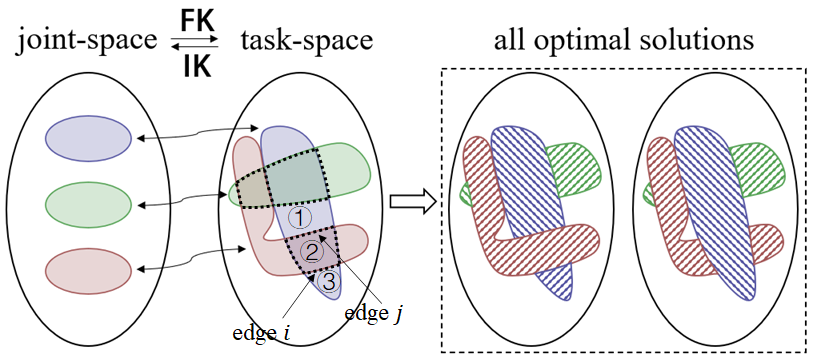
\includegraphics[width = 0.48\textwidth]{figures/mapping_2}
\caption{A toy illustration of the problem arising when planning optimal non-revisiting coverage paths with a manipulator: valid robot configurations form disjoint sets in joint-space, while their task-space FK mapping images (end-effector poses) may overlap. 
%, which is the key problem to be solved for non-repetitive CPP task. 
In the example, which for simplicity is illustrated with cells that are maximally $2$-overlapped, the resulting task-space graph 
% we don't really show the full graph, but will get complex, so we show snippets. I think clear like this.
%\textcolor{blue}{It is the initial graph (in the ``task-space" ellipse), and the right two graphs are the only } 
conveys $N = 11$ undetermined edges constructed as shown by the dashed lines, thus separating the graph into $M = 11$ cells.
To facilitate the understanding whilst limiting clutter in the graph, 3 cells and 2 edges ($i$ and $j$ in dashed blue-green and blue-red respectively) are singled out.
Solving the NCPP problem for the set of edges in the example can easily reveal all the optimal solutions in this case (two, depicted), demarcating the minimal bound for lift-offs as four. 
%\textcolor{red}{Tong, make sure this is 100\% correct; would a solid green split the solution into more lift-offs? we won't say, I want to say the above, but but pls make sure. No need to explain it to me, I just want a "Yes it is correct" answer, I can feel it to be the case, but have not expand the graph fully to be 100\% sure}.
%<ty> Yes, it is correct. 
It is easy to appreciate how as more colours ``intersect", the algorithmic complexity to find the optimal solutions will soon escalate (more intricate examples are provided in Section~\ref{section_experiment}). 
%note: can we lead here in the txt with a final comment where intuitively hint at the proposed solution by means of exploiting the topological 'intersections'? not sure we can do so clearly with this example, if you can, add a succint note here in that regard. Otherwise we simply present the problem of how complexity grows
It is also intuitive that should the green colour remain a complete set, both the red and blue colour cells would be split into further disconnected parts, leading to extra lift-offs. %so in order to get global optimality, the green colour must be sacrificed. 
This hints at the fact ``intersecting" colours %may be a \textit{topological invariance} of the graph that 
can be exploited to reduce the complexity of the solution.
}
\label{fig:mapping}
\end{figure}


%\subsection{Existing Solutions Revisiting}
% <ty> we may again propose the result in Tmech. See how many pages can be left for this. 

% \textcolor{red}{We should open up in more generic fashion, describing a wider range of alternatives in a small paragraph, then note the best, ours, as below}.

%\begin{color}{blue} See whether this paragraph perfectly covers the content of the next paragraph (citation will be added tomorrow, save time to modify algorithms) \end{color} 

Early reports on the generic \textit{coverage path planning} (CPP) problem focused on geometric path designing, particularly for mobile platforms operating in planar surfaces, such as boustrophedon~\cite{choset1998coverage} or spiral paths~\cite{hassan2018a}. 
Additional strategies were later proposed that transformed the coverable region into smaller partitions, or \textit{cells}, where continuous coverage paths could be guaranteed. A body of novel partitioning \textit{cellular decomposition} strategies emerged~\cite{choset2000exact}~\cite{huang2001optimal}, applied directly onto the area to be covered. This is an ineffective strategy when transferred from task to joint space for manipulator planning since the kinematic mapping between the two spaces is non-bijective: as illustrated in Fig.~\ref{fig:mapping}, the forward kinematic relationship from the configuration space to the surface is surjective (many-to-one) and locally flat (one-to-one from each connected component of the valid configuration space to the surface). 
The problem is further compounded when the end-effector can only visit each point on task-space once, leading to numerous pose reconfigurations during the motion of the end-effector~\cite{rososhansky2011coverage}.
%extended the results to more complex scenarios, providing a complete solution~\cite{}. 
%leading to significant gains towards overall smoothness in the resulting manipulator paths~\cite{}. 
%A body of novel partitioning \textit{cellular decomposition} strategies extended the results to more complex scenarios, providing a complete solution~\cite{}~\cite{}. 
%This is an adequate constraint for mobile robot navigation assignments for instance~\cite{}, but does not translate well for manipulator CPP tasks~\cite{} operating in joint-space, not in the task-space, 
% I comment out the below, not in context, non-dedundant single manip NCPP
%\textcolor{blue}{Since the problem is intrinsic to the manipulator kinematics and is unavoidable when the manipulator do not have redundant joints, using multiple manipulators~\cite{Kabir2019Generation}, redundant manipulators~\cite{} or mobile manipulators~\cite{Atkar2003Towards} have to be the last-resort solutions of the NCPP task. 
Many criteria in the classic CPP problems have been adapted to the manipulator NCPP task, such as time to completion~\cite{lu2020time} or energy consumption~\cite{mei2004energy}, and optimal mobile manipulator pose for a given coverage in task-space has also been investigated~\cite{paus2017a}. However, optimising  end-effector lift-offs for increased smoothness and continuity has been rarely exploited. %, which significantly reduces the time and energy consumption during manipulator reconfiguration.}
Recent propositions in the literature to tackle the problem decomposed the task-space area into a %initial 
topological graph ensuring continuous joint-space coverage within each cell, and looked for solutions where maximal continuity between cells existed~\cite{Yang2020Cellular}, as intuitively depicted in Fig.~\ref{fig:mapping}. 
%\textcolor{red}{our other works too? maybe too much as NO other CPP manip. refs!}
%\textcolor{blue}{Do you mean that we simplify the description of Tmech paper and add content to other manipulator paper? See whether now it is OK. }
All maximal-continuous cellular decompositions were proven to be collectable in a finite number of steps, defined by edges that represent the smallest, inseparable elements and cells that could only have a finite number of different sub-divisions.  

%\textcolor{red}{ Recent propositions in the literature formulate a solution in two stages, an initial optimal cellular decomposition at its core, which can then be followed by an arbitrary coverage path planning routine (\textcolor{red}{ref boust., or spiral, ...)} within each cell~\cite{Yang2020Cellular}. As a result, the problem is thus transformed into an optimal matching of each point on the surface to one of its IK solutions under a continuity constraint. Representing different sets of joint-space configurations as different colours, a point on the surface can be painted with multiple colours (see Fig.~\ref{fig:mapping}). The cell, a region of task-space contiguous points, is defined as a maximal connected region in which all points can be painted with same set of possible colours.} 

This is however an intensely computational process, growing exponentially in the size of the graph. Let there be $M$ topological cells and $N$ internal topological edges in the modelled graph to be solved. The number of edges for the $i$-th cell is $\alpha_i$, and denote the number of possible colours to fill cell $i$ as $K_i$.   
It has been shown how a binary array of length $\alpha_i$ can be used to index all possible different divisions of cell $i$~\cite{Yang2020Cellular}, whereby 
%$0$ at the $r$-th position enforcing the cell having different color to its $r$-th adjacent cell, while $1$ enforcing a same choice of colour. 
$0$ at a given position enforces the cell having a different color to its adjacent cell, whilst $1$ compels the same choice of colour. 
However, as supported by the illustrative example shown in Fig.~\ref{fig:many_to_one} for one of the edge solutions $(1111)$ and $2$ possible colours available for painting, the binary array does not uniquely represent a valid painting solution: the cell may be divided into two parts with differing colours, while each part themselves connect to their two adjacent cells. Following the cell sub-divisions, $4$ valid painting solutions of this cell appear corresponding to the edge solution $1111$. 
%An example of this is illustrated in Fig.~\ref{fig:many_to_one} . 
%\textcolor{red}{we don't show what the adjacent colours in the example are, so does this matter? would it be the same for 0000, or 0001 ...? don't provide a long explanation to me pls, try to think like a reade who has NEVER seen [1], and finds this all of a sudden. We are trying to use it to explain the complexity of the problem, and how to improve it. Nothing more. Would he get this from reading this explanation and Fig 1? not sure. We need Fig 1 to explain the complexity issue below, it MUST stay, and I like the caption. But from the drawing and the explanation, I don't think the reader can relate this to the earlier Fig 1, where the problem is clearly defined and teh concept of cell and topological edge also I believe is clearly estated and defined).}
%The enumeration of a single cell is executed on all cells to find all optimal solutions.
%\textcolor{blue}{This note is for which definition? }\textcolor{red}{??? ``The enumeration of a single cell is executed on all cells'' : this unncessary enumeration is the key to our proposed improvement, but from that single sentence droped out of context is not possible to see - what is the problem here? you make a statement, mathematically correct, but why that is a problem is not expressed. You need to "lead", explain with common language, not just drop things like these ...}
%\textcolor{red}{Since every two adjacent cells share a same edge, the overall number of elements to be enumerated is the number of internal edges (the edges on the boundary of the coverable area cannot be ``connected"). For simplicity, we approximately say it is ``all edges", which makes no difference to the contribution of this work because the term containing $N$ will be totally removed in this paper. --- you can't say this, makes not sense, if it makes no contribution and ``will be removed'', whay is it there in the first place!!??}
%While this has been proven a finite exercise~\cite{Yang2020Cellular}, it comes at a significant cost. 

\begin{figure}[t]
\centering
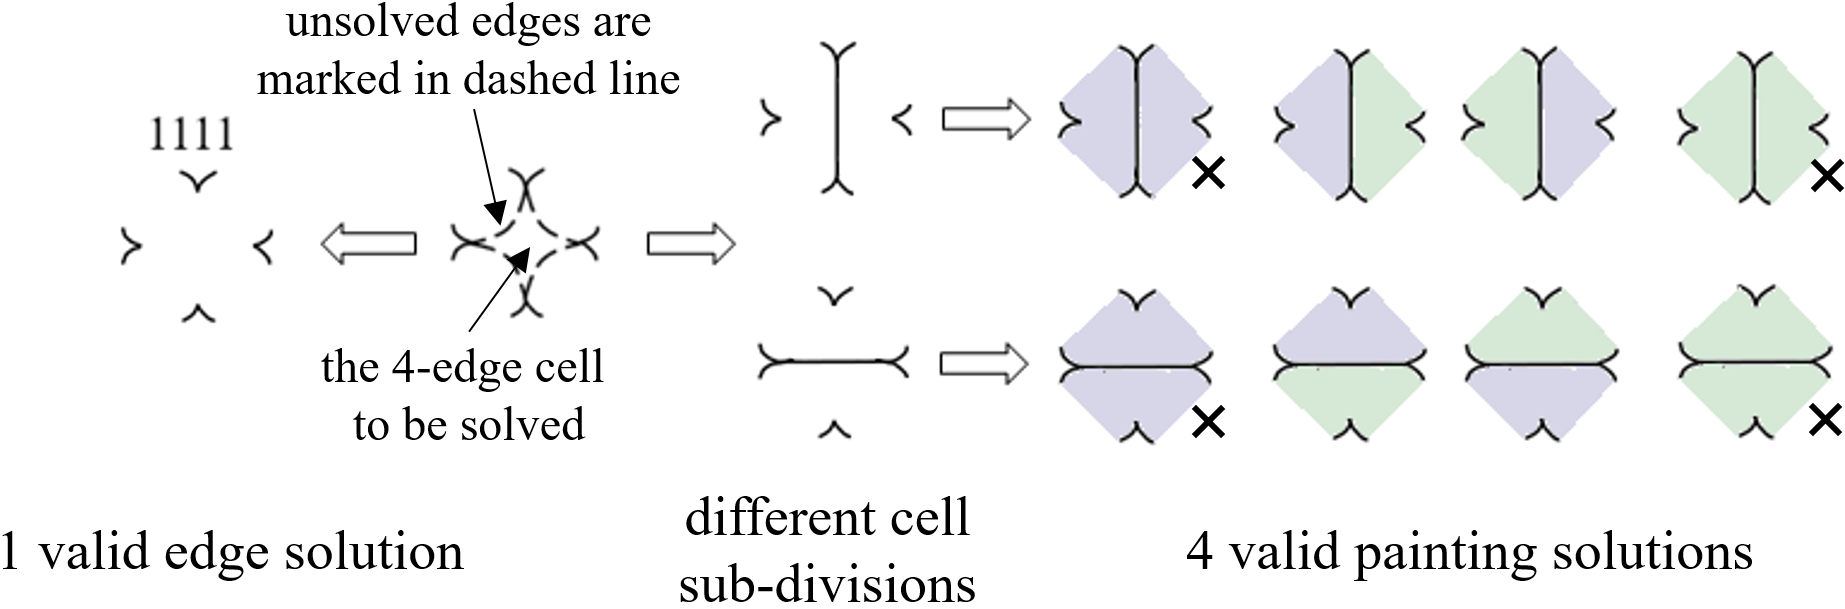
\includegraphics[width = 0.48\textwidth]{figures/many_to_one_3}
\caption{An illustration of the many-to-one relation between edge and painting solutions. 
Let a cell with $4$ adjacent cells (a $4$-edge cell) have 2 possible colours ``blue" and ``green", then $\alpha = 4, K = 2$. From the point of view of solving edges, the binary number $1111$ specifies one solution, but the corresponding valid painting solutions are multiple, $4$ to be precise: there are $E=2$ ways to divide the multi-edge cell into $3$-edge sub-cells, and $\alpha-2 = 2$ sub-cells are generated which can be filled with the $K (=2)$ possible colours. After enumerating $E\cdot K^{\max\{\alpha-2, 1\}}$ cases, four of them are removed (no subdivision when there is only one possible colour for all sub-cells), shown crossed-out, leaving the remaining four valid painting solutions.
}
\label{fig:many_to_one}
\end{figure}


\begin{comment}
Since every edge has two adjacent cells, 
the relation of $\alpha_i$ to $N$ is established by
\begin{equation}
N = \frac{1}{2}(\sum\limits_{i=1}^M \alpha_i - \tilde{N})
\end{equation}
($\tilde{N}$ simply denotes the number of edges on the outer boundary of the graph, %(with adjacent cells $-1$ ) 
which are determined and thus need not be enumerated). 
%Note that, although proving the finiteness of dividing each cell into sub-cells is enough for proving the finiteness of the whole process, the overall algorithmic complexity is far more than $2^N$, 
It has been shown in the Fig.~\ref{fig:many_to_one} counterexample how there is no one-to-one correspondence between the edge and painting solutions. 
The edge solution depicted, 1111, could be painted with 4 different valid painting alternatives.
Generically \textcolor{red}{is this from Tmech? I think so, so we need to reference it, not just drop it expecting the reader will be able to figure that out, not possible!} it has been proven by the cell sub-division strategy described in~~\cite{Yang2020Cellular} how if $\alpha_i \geq 4$, cell $i$ will be iteratively divided into $(\alpha_i-2)$ $3$-edge sub-cells\footnote{Here for simplicity we only consider the worst case presented in~\cite{Yang2020Cellular}. Beyond dividing fully into $3$-edge cells, the complexity of enumerating other cell sub-divisions is omitted \textcolor{red}{but it is also part of the enumeration of edges, shouldn't we? or you mean that taking the worst case, 4 adjacent cells, represents the highest computation and therefore we only need to consider this case for complexity calculation? - which I agree with}.}, and each sub-cell can be individually assigned with $K_i$ colours. Let there be $E_i$ different ways to divide cell $i$ into sub-cells, the overall complexity %\footnote{Here we disregard speeding-up tricks proposed in existing literature, because they are also valid in the algorithm proposed in this work. } 
can then be calculated as
\end{comment}

There is a need to enumerate all the edges for each cell, leading to all different colours to be subsequently filled in to create all posissible solutions~\cite{Yang2020Cellular}. This is a costly exercise. For the more generic case % we need this precision to figure out E_i
of a multi-edge ($\alpha_i \geq 4$) cell, other than the simple case of considering it as a whole, it may be sub-divided into up to $(\alpha_i-2)$ sub-cells, and each sub-cell can be individually assigned with $K_i$ colours. Considering a worst case scenario, let there be $E_i$ different ways to divide cell $i$ into $(\alpha_i-2)$ sub-cells, then $E_i\cdot K_i^{\max\{\alpha_i-2, 1\}}\cdot 2^{\alpha_i}$ steps are required for a single cell. Iteratively enumerating each cell and noting that each edge will only be enumerated once in the process, the algorithmic complexity can be calculated as
\begin{equation}\label{equ:tmech_complexity}
\prod\limits_{i=1\atop\alpha_i \geq 4}^{M}E_i\cdot \prod\limits_{i = 1}^M K_i^{\max\{\alpha_i-2, 1\}} \cdot 2^N
\end{equation}


\begin{comment}
Also note that as a dual graph of the commonsense ``node-edge" graph, the cells, edges and vertices correspond to the nodes, edges and faces (temporarily denoted as $F$ which has no usage in the NCPP problem), respectively. Then the relation of the number of cells $M$ and the edges $N$ is given by the Euler's formula for planar graph, 
\begin{equation}
N-M = F-2
\end{equation}
In a complicated graph we must have $F\gg 2$, then $N \gg M$. 
\begin{color}{blue}
We observe that enumerating an edge is a too trivial process to lead to different topologies of the resulting solution. See Fig.~\ref{fig:mapping}, where if edge $i$ is kept, then $j$ need not be removed, because even if cell \ding{172} and \ding{173} are connected, it makes no difference to the topology if cell \ding{174} is not connected together. 
In other words, existing works have avoided equivalent cellular decompositions under the equivalence of continuous modification of the cutting paths of cells. But looking at the topology of the resulting solution from a top-down view might further avoid carrying out equivalent multi-step processes in enumerative solving. 
In this paper, we introduce a high-level abstraction of the topology, the \textit{intersection}, which is the origin of the multiplicity of the optimal solutions. We show that intersections are unavoidable and have to be enumeratively solved. 
However, by separating the graph into intersection-free sub-graphs, all intersections are implicitly enumerated while sub-graphs are combined. As a result, the algorithmic complexity of enumerating all edges, $2^N$, is removed. 
\end{color}
\end{comment}

Careful examination of the topological graph leads in this work to the introduction of a high-level abstraction, the \textit{topologcal  intersection} which is the origin of the multiplicity of the optimal solutions. It is hereby proven that intersections are indeed unavoidable and have to be enumeratively solved. However, separating the graph into intersection-free sub-graphs leads to all intersections being implicitly enumerated when the sub-graphs are recombined later to calculate the final solutions. The end result is the removal of the substantial complexity in enumerating all edges, $2^N$. 


The remainder of this paper is organised as follows. Section~\ref{section_intersection} introduces the concept of \textit{topological intersection} and the \textit{intersection-free graph} property.
% and shows its vital role to solve simple graphs.
Section~\ref{section_graph_separation} describes concrete steps to separate a graph into intersection-free sub-graphs. 
Solutions to these can then be combined to construct the optimal solutions for the full graph as described in Section~\ref{section_full_graph}. Details  about the complexity advantage in solving the problem following the proposed strategy is mathematically proven in Section~\ref{section_complexity}, whilst experimental results from simulations are collected in Section~\ref{section_experiment}. Final concluding remarks are gathered in Section~\ref{section_conclusion}.

\begin{comment}
\subsubsection*{Notation}
\textcolor{red}{Not critical!ok as is. But pls make sure this clarification is absolutely necessary. If use sparingly later, or can be noted when first used, maybe best than here. Otherwise it is fine, we have bigger problems!} 
The word \textit{divide} refers to the division of a cell with a \textit{cutting path}, whilst a graph is \textit{separated} into multiple sub-graphs through a \textit{separating path}. Thus, \textit{cells being separated} means a graph is separated via dividing the specified cells into parts, then one sub-cell is connected to one sub-graph while the other sub-cell is connected to another sub-graph.  The variables $i,j$ and $n$ are used for indexing. 
\end{comment}

\begin{figure}[t]
\centering
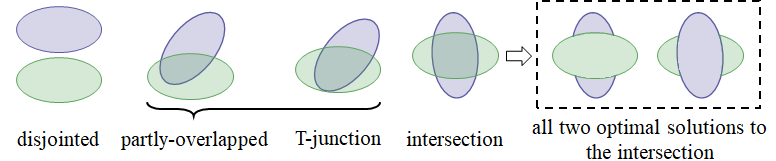
\includegraphics[width = 0.48\textwidth]{figures/basic_shape_3}
\caption{Illustration of basic relations between the reachable area of two colours. T-junction is a special case of the partly-overlapped distribution of colours, while it can be transformed back to a normal case through continuously modifying the boundary of colours. Only the intersected case needs solving, and it is apparent that the two optimal solutions are not topological equivalent, since they have the different number of connected regions in blue and green colour. }\label{fig:basic_shape}
\end{figure}

\section{Optimality via ``Topological Intersections''}
\label{section_intersection}
In this section, we introduce a topological invariant variable, \textit{intersection}, whose enumeration is the core element leading to notable inefficiencies in solving the full graph. The simplified representation of all solutions of an intersection-free graph is then made apparent.  


\begin{figure}[t]
\centering
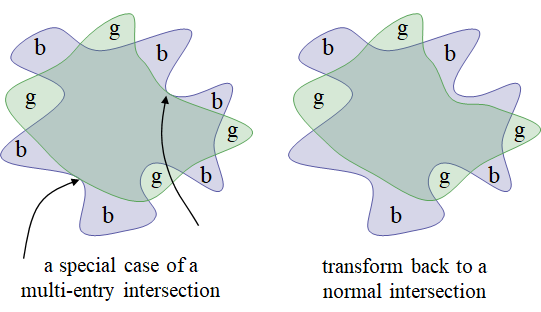
\includegraphics[width = 0.4\textwidth]{figures/multi_entry}
\caption{An intersection with $8$ entries. For some special cases that two consecutive adjacent cells can be filled in same colour, through shrinking the boundary of colour, it can be transformed back to the normal case. }\label{fig:multi_entry}
\end{figure}

\begin{figure*}[t]
\centering
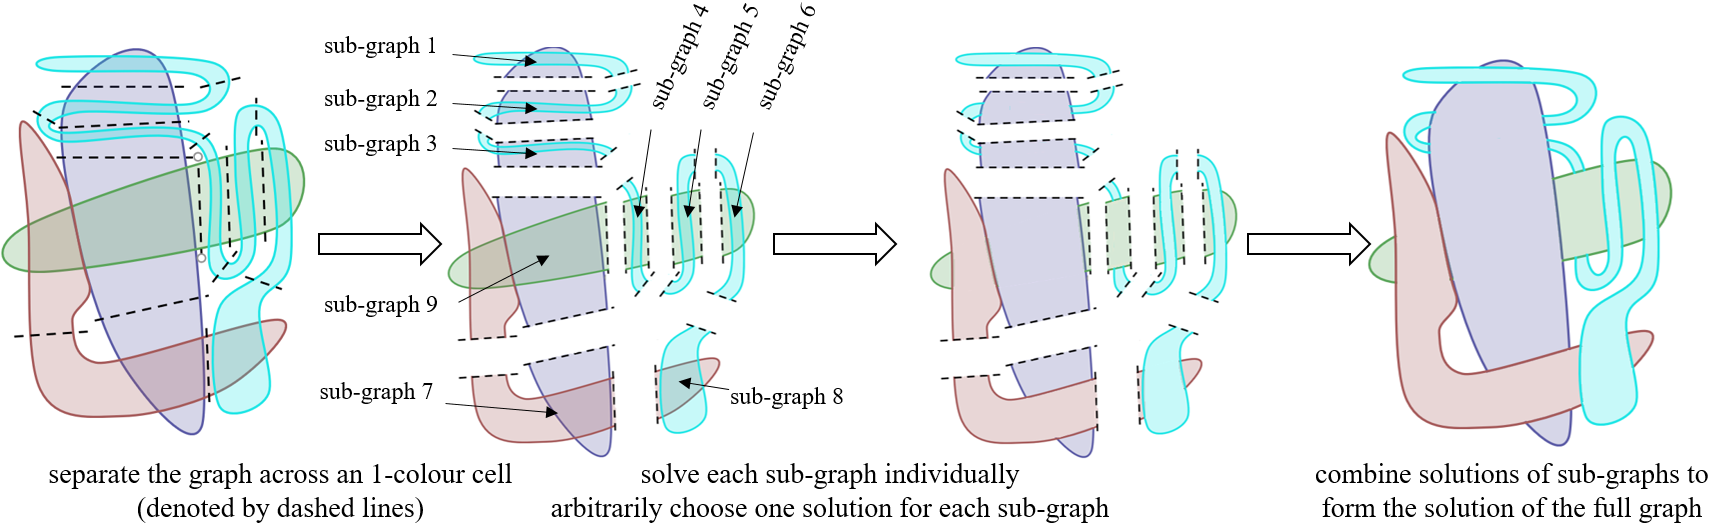
\includegraphics[width=\textwidth]{figures/two_overlapped_graph_2}
\caption{A maximally 2-overlapped graph to show the role of intersections. The full graph (left) is separated into $9$ sub-graphs through $1$-colour cells, shown with dashed cutting lines. Sub-graph $1$-$8$ has been shown to have two optimal solutions, while sub-graph $9$ gets a unique optimal solution after enumerative solving. Note that whatever solution gets chosen in each sub-graph, when two sub-graphs are combined, the two $1$-colour sub-cells separated by the dashed line re-join together, resulting in a reduction of one on the number of continuous regions. In total $4+(3\times 8)=28$ connected regions can be observed after solving the sub-graphs individually, combined with cost $-15$ (number of dashed lines). The nonrepetitive coverage problem of this graph ends up with $28-15=13$ connected regions, i.e., $12$ lift-offs. 
Note that no intersections in the full graph are avoided when solving all the sub-graphs. And different choices of the solution for each sub-graph will double the number of optimal solutions of the full graph: there will be $2^8=256$ optimal solutions to the graph.
}
%The number of continuous regions is $4+(3\times 8) = 28$  \textcolor{red}{??}, and $15$ dashed lines are created  \textcolor{red}{why? you say what you do, not why?}, so the number of continuous regions in the original graph is $28-15=13$, i.e., $12$ lift-offs are necessary to finish this coverage task. However, for all optimal cellular decompositions, each intersection has to be enumerated. The total number of optimal cellular decompositions will be $2^8 = 256$ \textcolor{red}{why?}, and no two of them are equivalent under continuous modification of cell boundaries \textcolor{red}{is this apparent in the figure? I can't see it}. 
\label{fig:two_overlapped_graph}
\end{figure*}


\subsection{Defining Intersections}
An intersection is a class of overlapping between the coverable region with two colours, describing an inevitable interruption of the connectivity of one colour 
by other colours. 
The coverable area of two colours may be fully disjointed, partly overlapped or intersected, as shown in Fig.~\ref{fig:basic_shape}, 
whereby colours can be both kept connected in the disjointed and partly overlapped cases, but critically in the intersection case one colour being connected will truncate the other colour into two parts. 
And obviously, there are two optimal solutions to this intersected case, filling in the central cell full of either blue or green.
%Either colour being connected is obviouly an optimal solution. 
%\textcolor{red}{you mean in isolation, as shown in the fig? below you make the case for more complicate graphs, but here you don't}  
In more complicated graphs, such an intersection may introduce two sets of optimal solutions, in one set all solutions keep one colour connected, 
while in the other set the other colour remains connected. Seeing the intersection in Fig.~\ref{fig:basic_shape} as $4$ entries, the intersection with arbitrary number of entries is intuitive, as shown in Fig.~\ref{fig:multi_entry}. After simplifying the intersection by merging consecutive adjacent cells which have the same set of possible colours, the intersection will have $n$ (an even number) entries. 
It is observed that for each adjacent cell (say the $i$-th, labelled cyclicly), if it is connected to any other adjacent cell through an intersection, then another two entries, $(i-1)$ and $(i+1)$, cannot be connected. So the minimal number of continuous regions for an $n$-entry intersection is $\frac{n}{2}+1$. 
However, note that even if the optimal number is directly deduced, we still have to enumeratively solving the intersection to get all optimal cellular decompositions. 
\begin{comment}
Denote the cyclic sequence of adjacent cells of an $n$-entry intersection by 
\begin{equation}
\mbox{intersection}_n = [g_1 b_1 \cdots g_i b_i \cdots g_{\frac{n}{2}} b_{\frac{n}{2}}]
\end{equation}
where ``b" and ``g" represent colour ``blue" and ``green", the iterative enumeration can be represented as 
\begin{equation}
\begin{aligned}
\mbox{solution}_n =& \{[g_1 b_1 \cdots g_i b_i \cdots g_{\frac{n}{2}} b_{\frac{n}{2}}]\}\\
=& \{[g_1 b_1 \cdots b_{i-1}(g_i) b_i \cdots g_{\frac{n}{2}} b_{\frac{n}{2}}]\}\\
&\cup \{[g_1 b_1 \cdots b_{i-1})g_i( b_i \cdots g_{\frac{n}{2}} b_{\frac{n}{2}}]\}\\
=& \{g_i, [g_1b_1\cdots g_{i-1}b_{\{i-1, i\}}g_i\cdots g_{\frac{n}{2}}b_{\frac{n}{2}}]\}\\
&\bigcup\limits_{j \neq i} 
\end{aligned}
\end{equation}
where $(\cdot)$ represents dis-connectivity of elements. 
\end{comment}
For the $i$-th entry, we will separately consider (a) connecting it to other entries, or (b) keeping itself disconnected so that entries $(i-1)$ and $(i+1)$ can be connected. Both of them go to optimal cellular decompositions. 





\begin{comment}
\subsection{Solution of Maximally $2$-overlapped Graph}
\textcolor{red}{note: is this provided for illustration only with a smaller problem? we then move on to the width-2 strip sub-graphing, that is the actual final solution. Correct? If so, we should intro this differently. }
\textcolor{blue}{Yes, the divide-and-conquer strategy cannot be used when there is no $1$-colour cell to separate. We just use it to show that intersections are unavoidable and we have to proactively solve them. (and in the next section we will show that, when separating graph through multi-colour cells, the ``solving" of intersections has to be ``enumeration". )
} 
\end{comment}


The core role of intersections in graphs can be revealed in solving a simpler case, a separable maximally $2$-overlapped graph, 
illustrated by Fig.~\ref{fig:two_overlapped_graph}.  
%Here we provide an efficient \textit{divide-and-conquer} solution to the maximally $2$-overlapped graphs (for each cell, there are at most $2$ possible colours). 
%The efficiency of the solution is intrinsic to the uniqueness of colour of the cell to be separated. 
The key step is to separate the graph into sub-graphs by dividing $1$-colour cells connecting intersections. 
%The dashed lines are the places where we separate the original graph into sub-graphs. 
Since the divided cell only has a unique coverable colour, we divide one cell into two unconnectable cells (they belong to different sub-graphs), so the number of continuous regions on the graph should be the sum of continuous regions in sub-graphs minus the number of dashed lines. 
Moreover, we can arbitrarily combine the optimal solutions of sub-graphs to form the optimal solution of the original graph. 
However, it should be noted that while the computational cost of combining solutions of sub-graphs has been reduced, no intersection was removed. 
Intersections must be solved within the sub-graphs, and all optimal solutions collected through a full combination of the different solutions with 
intersections, as further described in Section~\ref{section_full_graph}.
% <ty> We don't give a separate subsection for this. I put this in the intro of Section "Graph Separation"

%\subsection{Local Property of Intersections}
There are a number of interesting local properties in the concept of graph intersecting. 
Fig.~\ref{fig:two_overlapped_graph} (sub-graph $9$) illustrates the case where two parallel (nonoverlapping but touching) colour region exist which are simultaneously crossed by a third colour. In this case, the graph cannot be trivially separated since the multi-colour cells are adjacent, with no $1$-colour cell in between. The generalised cases of intersections that can be encountered are shown in Fig.~\ref{fig:three_overlapped_graph}. 
%The crucial observation of parallel regions and intersection is that they describe local distribution of colours but not a global characteristic between colours: two colours can be intersecting in a part of the graph, whilst remaining parallel in another part of the graph \textcolor{red}{isn't that a triviality? all options are possible - if we state something, is to lead towards an informative comment of how that affects our algorithm, or how to solve it, or ... not just state the obvious}. 
It is apparent how as more colours get involved, %, such as the case shown in Fig.~\ref{fig:three_overlapped_graph}, 
intersections become highly coupled, and even identifying intersections is not trivial. 
There is certainty in the fact that the number of intersections in a partly-solved graph will not reduce under continuous modification of cell cutting paths. 
Disregarding the position of intersections and how to solve them leads to exhaustive implicit enumeration when all edges and cells are enumerated~\cite{Yang2020Cellular}. 
On the other hand, exploiting the interesting complex scenarios that analysing the topology between different colours offer will attenuate this problem. In this regard, the concept of intersection-free graphs described next will play a crucial role.  
%, thus \textcolor{red}{thus? you can deduce the following statement from the prior? if you do, good, I can not see it, I rephrase as is assuming "thus" is correct, pls make sure} all intersections are implicitly reduced when all edges and all cell colours are enumerated.  
%\textcolor{blue}{No understanding of the position of intersections and how to solve the intersections will lead to a clueless exhausted enumeration, hoping that all intersections can be implicitly enumerated with all edges and all cells are enumerated, which is proposed by existing work~\cite{Yang2020Cellular}. To release the problem, properties of intersection-free graphs need to be exploited, which is given in the next subsection. }

\begin{figure}[t]
\centering
%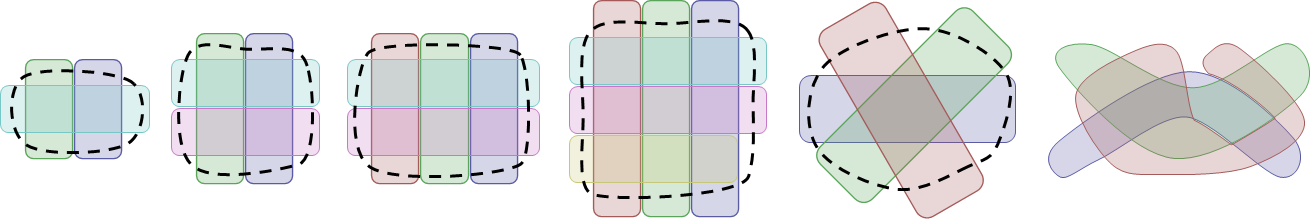
\includegraphics[width = 0.48\textwidth]{figures/three_overlapped_graph_2}
\subfigure[]{
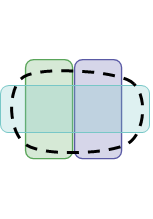
\includegraphics[height=0.06\textwidth]{figures/1_2_intersection}
}
\subfigure[]{
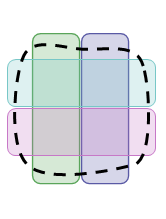
\includegraphics[height=0.06\textwidth]{figures/2_2_intersection}
}
\subfigure[]{
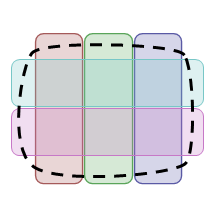
\includegraphics[height=0.06\textwidth]{figures/2_3_intersection}
}
\subfigure[]{
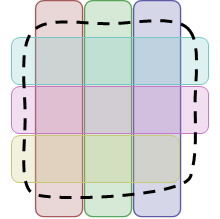
\includegraphics[height=0.06\textwidth]{figures/3_3_intersection}
}
\subfigure[]{
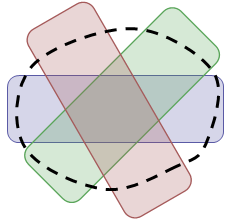
\includegraphics[height=0.06\textwidth]{figures/3_intersection}
}
\subfigure[]{
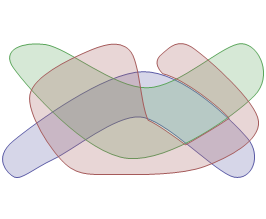
\includegraphics[height=0.06\textwidth]{figures/3_intersection_2}
}
\caption{Demonstrating graphs with various forms of intersections. 
The dashed circle marks a part of the graph which contains intersections. 
Intersection formed by: (a) $2\&1$ parallel colours, (b) $2\&2$ parallel colours, (c) $2\&3$ parallel colours and (d) a further special case of $3\&3$ parallel colours (where whether the orange colour intersects with the blue colour is closely related to the optimal solutions. Now they only form a T-junction), (e) a normal $3$-overlapped intersections and (f) a complicated $3$-overlapped graph which we cannot even figure out where is the intersection given too many intersections and parallels of colours in it. }\label{fig:three_overlapped_graph}
\end{figure}

%In this section, we introduced a topological invariance of an unsolved graph, intersections. 
%An efficient solution of maximally $2$-overlapped graph is proposed to reveal the significant role of intersections in solving a generic graph. 
%The number of intersections is shown invariant under homeomorphic modification of cellular decompositions while a valid cellular decomposition is free of intersection, so all intersections have to be iteratively solved. 
%In the next section we will show that intersections cannot be solved locally, then the process to remove an intersection has to be ``enumeration all cases". 
%However, such efficient solution cannot be generalized to arbitrary graph separation, as separating graph through multi-colour cells cannot be arbitrarily combined. the key step to improve the efficiency is to address the redundant steps of enumerating intersections, which is the main focus of the next section. 


\begin{figure}[t]
\centering
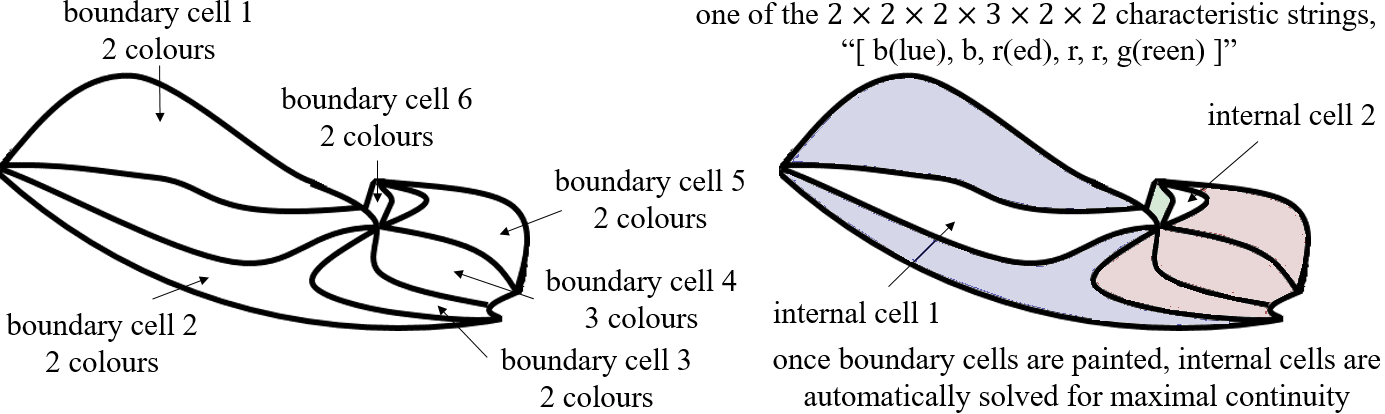
\includegraphics[width=0.48\textwidth]{figures/characteristic_string}
\caption{An intersection-free graph. The internal cell $1$ will choose blue $>$ green $>$ other colours. The internal cell $2$ will choose green $=$ red $>$ other colours.}\label{fig:characteristic_string}
\end{figure}

\subsection{Intersection-Free Graphs}

An intersection-free graph is a graph where no intersection can be constructed within it. Two types of cells can be distinguished in an intersection-free graph, a \textit{boundary cell} which has edges forming the boundary of the graph, and the remaining \textit{internal cell} which has no edge exposed to the graph boundary. It is apparent that all internal cells are shown to have less than $4$ cells, or else an intersection could be constructed within. 
See Fig.~\ref{fig:characteristic_string} for an illustration of the intersection-free graph with $6$ boundary cells and $2$ internal cells. 

A crucial property of intersection-free graphs is that the connectivity of the graph can be uniquely characterised by the colour of the boundary cell. 
To prove this, let the colour of all boundary cells be determined. On picking up two boundary cells with the same colour one must be able to judge their connectivity through this graph. Should connectivity be undetermined, one may find another pair of boundary cells whose connection may prevent these two edges being connected. However, this represents an intersection, which contradicts the assumption of intersection-free property of the graph. 

The colour of the (ordered) boundary cells can be recorded in a string with length equalling the number of boundary edges of the graph, referred to as 
the \textit{characteristic string} of the graph. After assigning a colour to each boundary cell, all internal cells will be assigned the colour which maximises 
the connectivity to their adjacent cells. 
After all cells have had their colour allocated, all the internal edges can be  automatically solved. 
It can thus be said that each characteristic string uniquely corresponds to a unique solution of the intersection-free graph, 
and the number of characteristic strings can then be liken to the full quantification of the number of solutions in the graph. 
\begin{figure}[t]
\centering
\subfigure[]{
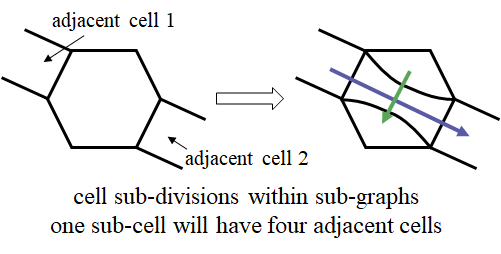
\includegraphics[width=0.22\textwidth]{figures/constraint_violation_a}
}
\subfigure[]{
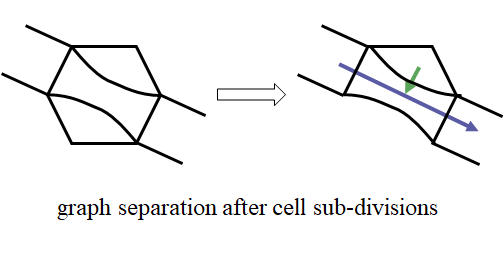
\includegraphics[width=0.22\textwidth]{figures/constraint_violation_b}
}
\caption{(a) Illustration of constraint violation due to cell sub-divisions in sub-graphs. (b) If a cell is scheduled to be divided, it should first be divided and the followed by  constructing the intersection-free sub-graphs.}
\label{fig:constraint_violation}
\end{figure}

\section{Graph Separation}
\label{section_graph_separation}
%This motivates us to find a novel topological structure called \textit{width-$2$ strip}, or \textit{strip}, which is proven intersection-free. 
%With the graph being separated into strips and each strip being solved individually, we combine all solutions of strips to generate all solutions of the original graph, where all optimal solutions are included. 
%\textcolor{blue}{We might put this sentence to conclusion of this section: 
%Recall that intersections are intrinsic to the graph, non-existence of intersections in strips means that all intersections are automatically solved while strips are combined, which do not add extra algorithmic complexity. 
%}
 An efficient strategy to separate a graph into intersection-free sub-graphs is described in this section. 
Since non-adjacency of internal cells in sub-graphs will be enforced, and cell sub-division after sub-graphs have already been constructed, 
this constraint may be violated (see Fig.~\ref{fig:constraint_violation} for an illustration of this scenario).
So let at this point all $n(\geq 4)$-edge cells have been properly divided before applying the algorithm, 
thus all cells in the sub-graphs can only be seen as a whole and be filled with the same colour. 
An apparent result from this is that the graph should not be separated across edges, or else the constraints of the original cell vanishes, and non-optimal solutions may appear. See an illustration of this scenario in Fig~\ref{fig:separation_at_edges}. 
Another result is that the optimality of part of the graph has no relation to the global optimal solution of the whole graph. 
This is proved by the example illustrated in Fig~\ref{fig:local_combined}. 

\begin{figure}[t]
\centering
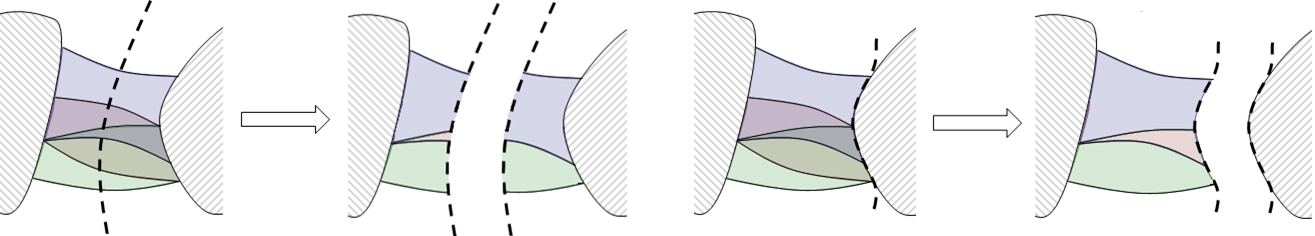
\includegraphics[width=0.48\textwidth]{figures/separation_at_edges_2}
\caption{If a graph is separated through division of multi-colour cells, the constraint of the cell vanishes, then in the sub-graphs there may exist solutions that after being combined is non-optimal, such as the case given in left. If the graph is separated along edges, we will not incur such problem. }\label{fig:separation_at_edges}
\end{figure}


%\subsection{Relation between Optimality of Graph and Its Sub-Graphs}
%Before we go into relations between graph and sub-graphs, we have to claim a basic criteria for separating a graph into sub-graphs. 
%Different from separating the graph through an $1$-colour cell, where the solutions of sub-graphs can be arbitrarily combined, if we separate the graph through multi-colour cells, as illustrated in Fig.~\ref{fig:separation_at_edges}, the constraints of the original cell vanishes, then proven non-optimal solutions may appear. In contrast, separating the graph through existing edges has the same effort, which is desired. 
%So in sequel our graph separation process should  follow existing edges in the graph, which makes Fig.~\ref{fig:non_optimal_subgraph} and Fig.~\ref{fig:local_in_other_graph} reasonable. 

%It is also observed that if the edge has multi-colour adjacent cells, then the combination of different solutions of sub-graphs will have non-trivial cost variation (not $-1$ as used in Fig.~\ref{fig:two_overlapped_graph}). 

\begin{figure}[t]
\centering
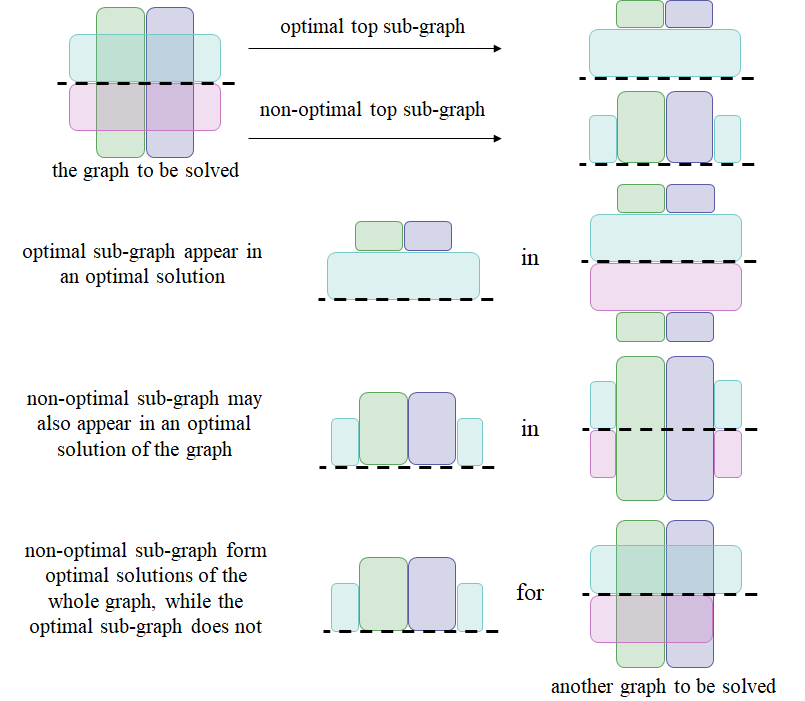
\includegraphics[width=0.48\textwidth]{figures/local_combined}
\caption{Separating the graph through the dashed line, we show the optimal solution and a non-optimal solution of the sub-graph. It is noticeable that both of them form optimal solutions of the original graph. An in the bottom case, as a sub-graph of another graph, the non-optimal sub-graph can form optimal solutions while the optimal sub-graph cannot do so. }\label{fig:local_combined}
\end{figure}

%\begin{figure}[t]
%\centering
%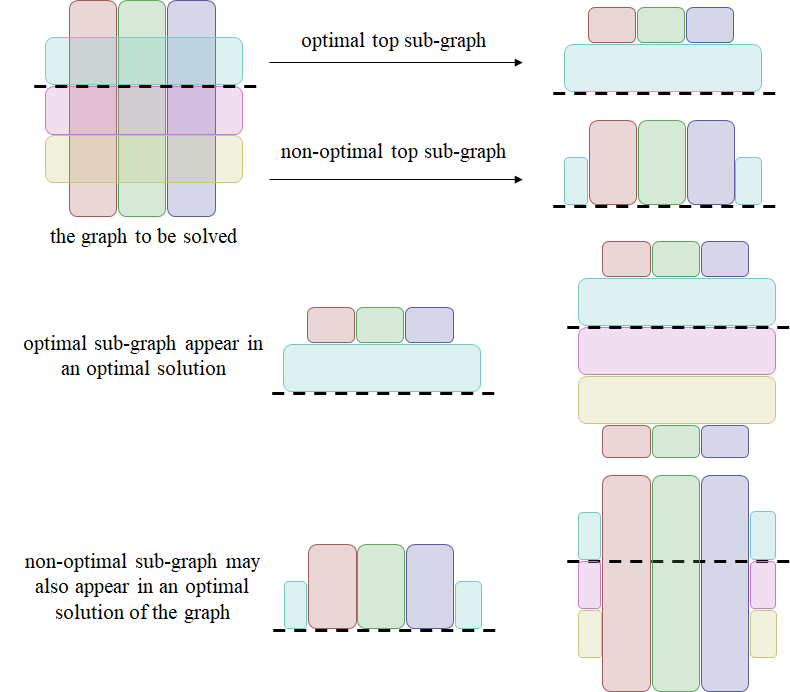
\includegraphics[width=0.44\textwidth]{figures/local}
%\caption{Separating the graph through the dashed line, we show the optimal solution and a non-optimal solution of the sub-graph. It is noticeable that both of them form optimal solutions of the original graph. }\label{fig:non_optimal_subgraph}
%\end{figure}
%
%\begin{figure}[t]
%\centering
%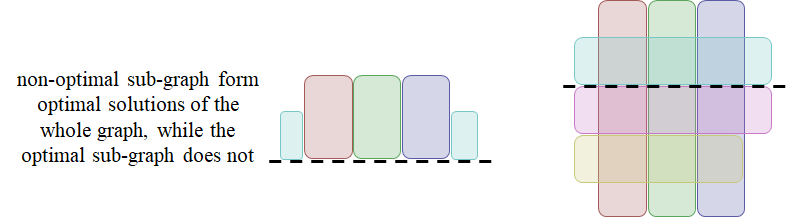
\includegraphics[width=0.44\textwidth]{figures/local_in_other_graph}
%\caption{Another graph to be solved which has the same sub-graph as the case shown in Fig.~\ref{fig:non_optimal_subgraph}. The optimal solution consists of only the non-optimal sub-graph but not the optimal sub-graph. }\label{fig:local_in_other_graph}
%\end{figure}

%Then, we claim that there is no guarantee about the global optimality of combining optimal solutions of sub-graphs. In other words, when a graph is separated into sub-graphs, we have to collect all solutions of each sub-graph. (It is not a bad thing if all solutions of sub-graphs can be enumerated, since in this case solving sub-graphs is unnecessary. )
%This is proved by two examples illustrated in Fig.~\ref{fig:non_optimal_subgraph} and Fig.\ref{fig:local_in_other_graph}. In \ref{fig:non_optimal_subgraph} both optimal and non-optimal solution of the sub-graph will form an optimal solution of the original graph. And in Fig.\ref{fig:local_in_other_graph} it is shown that non-optimal sub-graph is included in optimal solution of the original graph while the optimal sub-graph is not. 
%See Fig.\ref{fig:non_optimal_subgraph}, where the graph to be solved is an intersection between three parallel colours and another three parallel colours. The optimal solution is obviously either connecting all horizontal colours or connecting all vertical colours. 
%We can see from this case that optimality of the sub-graph is not equivalent to the optimality of the whole graph. So if a graph is separated into sub-graphs, we should store all solutions of sub-graphs but not only optimal solutions. 
%Another problem is that the optimality of a solution of the sub-graph hugely depends on other sub-graphs. A case is given in Fig.\ref{fig:local_in_other_graph}. 
%So we can only judge the optimality after we pick one solution from each sub-graph and combine them to form a solution of the whole graph. 
%In other words, in the absense of arbitrary combination of the solutions of sub-graphs, the algorithmic complexity of the graph is the multiplication but not the sum of the complexity of solving each sub-graph. 

%\begin{figure*}[t]
%\centering
%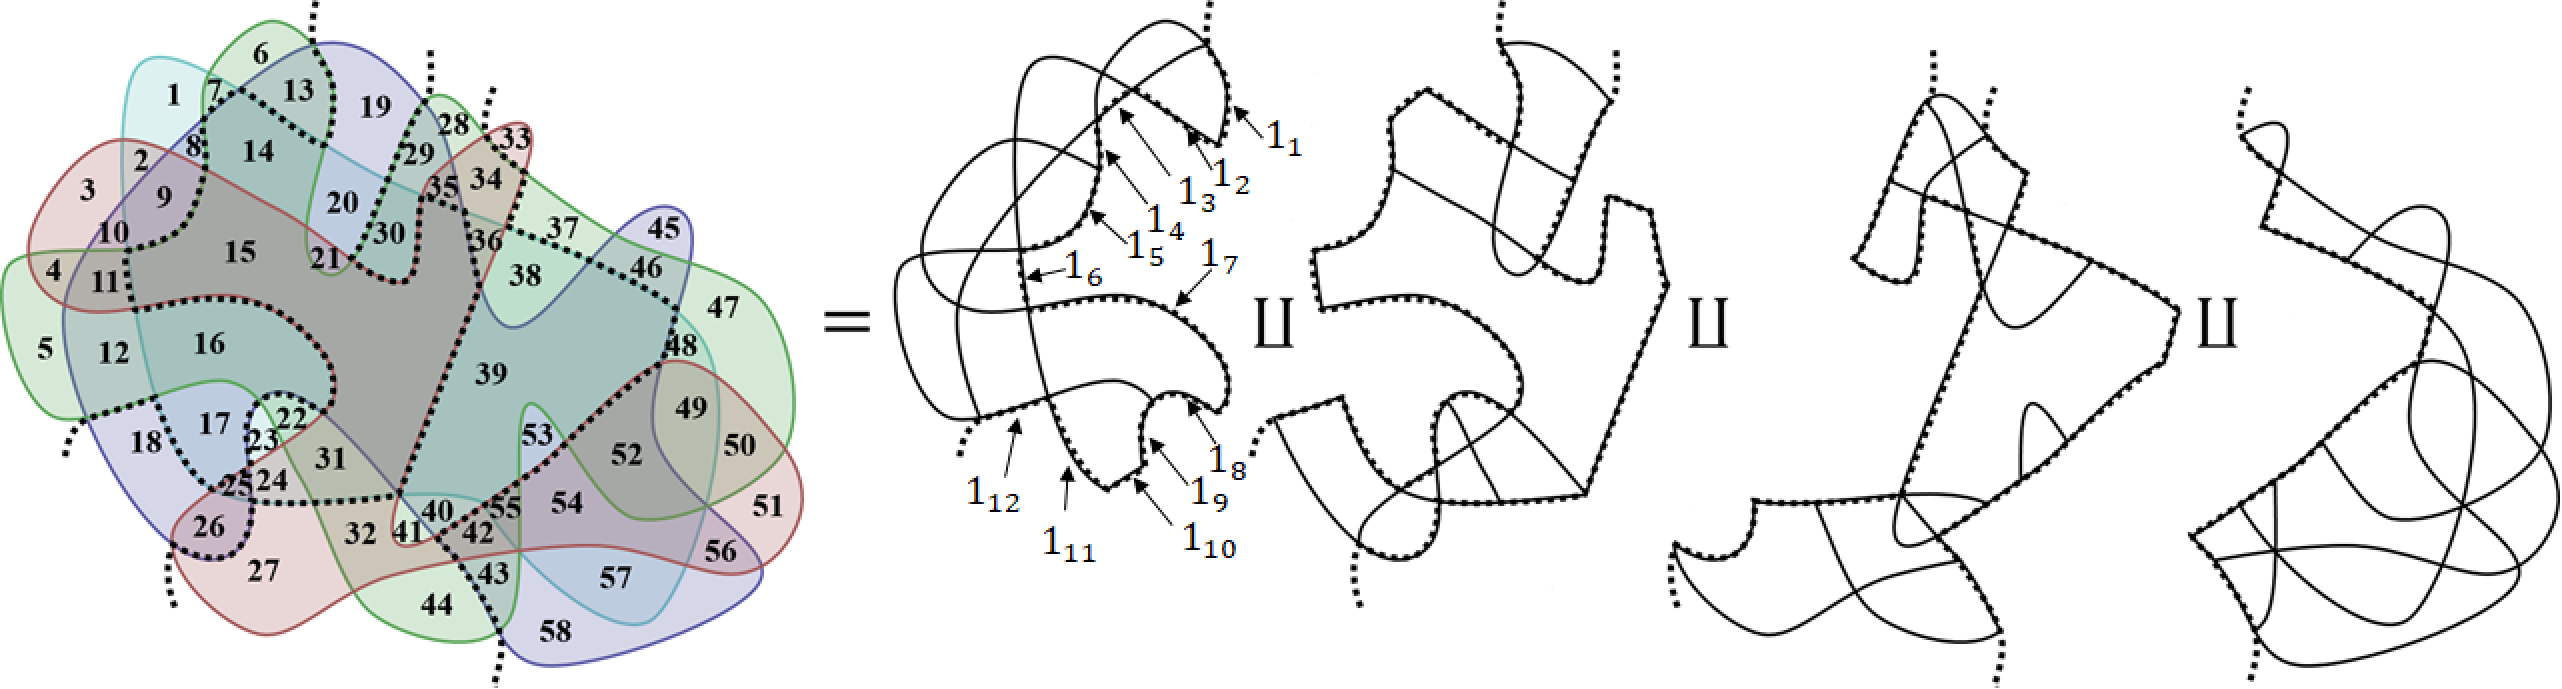
\includegraphics[width=0.96\textwidth]{figures/complicated_graph/graph_separation_with_index}
%\caption{\textcolor{blue}{TODO: divide some multi-edge cell into triangles as is done in experiment. }A demo graph with $4$ colours and $58$ cells. The coproduct sign $\coprod$ means that collecting all solutions of different sub-graphs are totally independent. It is easy to verify that there is impossible to form any intersection in each sub-graph. Then, the boundary characteristic uniquely corresponds to a cellular decomposition of the sub-graph. Note that the graph separation is not unique, and we only need a valid one. }\label{fig:complicated_graph}
%\end{figure*}

\begin{figure*}[t]
\centering
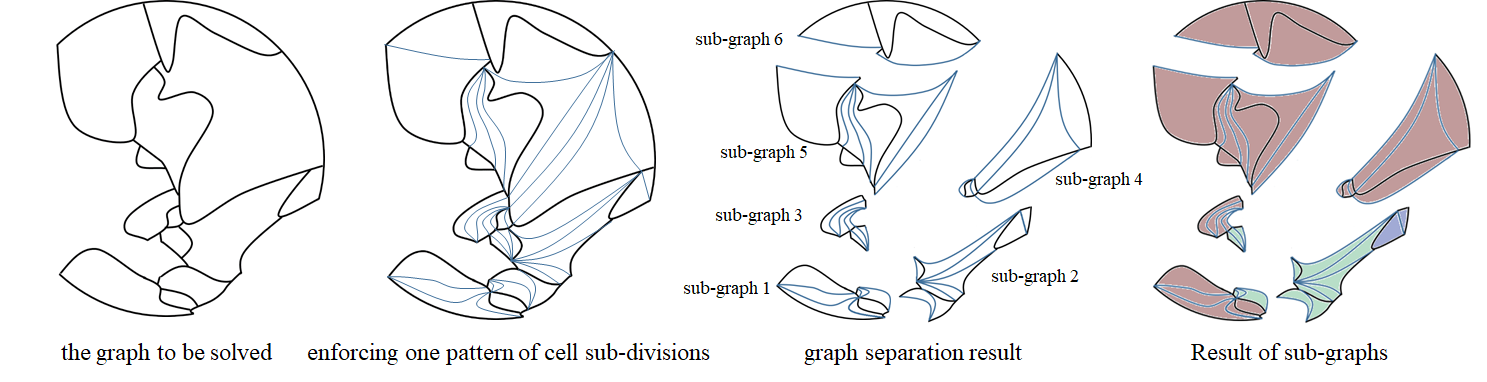
\includegraphics[width =0.96\textwidth]{figures/graph_separation_2}
\caption{Illustration of how an unsolved graph is separated into sub-graphs. }\label{fig:complicated_graph}
\end{figure*}

\begin{figure*}[t]
\centering
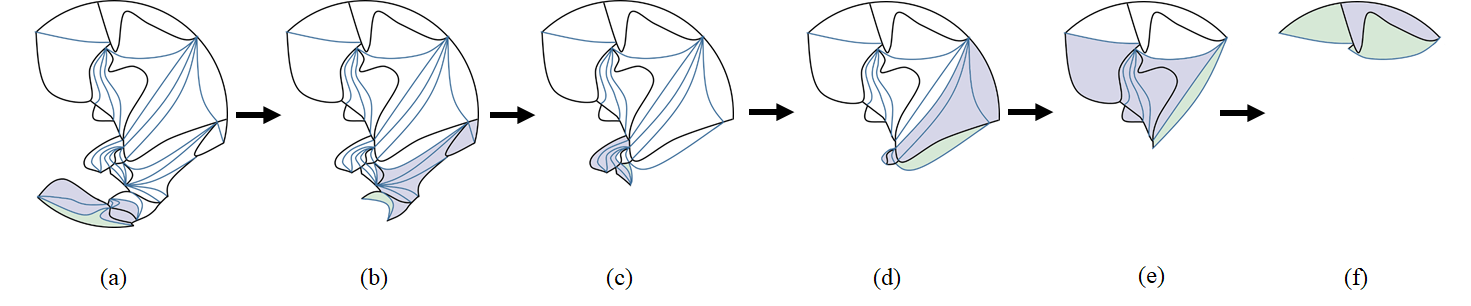
\includegraphics[width=0.96\textwidth]{figures/steps}
\caption{The concrete steps to separate the graph given in Fig.~\ref{fig:complicated_graph} into intersection-free strips. }\label{fig:steps}
\end{figure*}


\subsection{Defining Strips}
It is observed that when a part of the graph contains an intersection, there must exist at least $4$ entries. Moreover, each entry may not be a single edge.  
These motivate us to consider its opposite: if in the sub-graph it is enforced that (1) each cell has at most $3$ adjacent cells, then it can not possibly be an intersection. In noting that two internal $3$-edge cells may form a $4$-edge cell which breaks this criterion, it is enforced that (2) the internal cells are nonadjacent. 
A topological graph satisfying the above two constraints is referred to as a \textit{strip}. 


\subsection{Graph Separation into Strips}
%The discussion is given on a complicated example shown in Fig.\ref{fig:complicated_graph}, which is computationally unaffordable if we enumerate all edges and cells. 
%Following our assumptions, 
At this point in the start of the separation process it can be safely assumed that all multi-edge cells have been divided. % before starting graph separation. 
Please refer to Fig.~\ref{fig:steps} for a visualisation of the separation process with an example. One boundary cell is first selected and regarded as an element of strip $1$, shown in green in Fig.~\ref{fig:steps}(a).
% <ty> I'm not sure whether you can understand the below, and whether it is necessary.
% yes, "some" is no good, we have to specify how, I go with what I understand 
%\textcolor{red}{Read! ok?}
%The initial cells for the first strip are selected such that no multiply-connected strips can be constructed from them. %which introduce unnecessary discussion.
%In general any small subset adjacent to a selection of contiguous boundary cells will be a valid choice. 
%A counter-example in this case would be choosing for instance all boundary cells, $1, 6, 19, 28, \cdots, 4, 3$. 
%It is easy to create valid separations, so we omit further discussion on the initial selection. 
%The cells are only selected at the boundary, so it can be seen of width $1$. 
Then, for each adjacent cell of the strip, we check whether accommodating this cell into the strip will violate the constraints discussed earlier. 
Otherwise it is inserted. 
When no further cells can be inserted, the construction of strip $1$ is deemed finished. 
In this example, as shown in Fig.~\ref{fig:steps}(a), adjacent cells are iteratively inserted to strip $1$ which are shown in blue. If one more cell is inserted, then the boundary cell $5$ (illustrated in detail in Fig.~\ref{fig:characteristic_string}) will become an internal cell which is adjacent to the internal cell $2$, so the construction of strip $1$ terminates.  
To construct strip $2$, we check one-by-one whether the cells adjacent to strip $1$ can be inserted. 
After that, all adjacent cells to strip $2$  are again checked and attempted to be inserted into strip $2$. 
%Then adjacent cells of strip $2$ are iteratively checked to be included. 
By iteratively considering adding the adjacent cells to the previous strip into the current strip and adding more cells satisfying the two constraints, 
the whole graph is finally separated into strips, as shown in Fig.~\ref{fig:complicated_graph} where the example graph is separated into $6$ sub-graphs. 

\subsection{Solving Sub-Graphs}
After the graph has been separated, all the solutions for each sub-graph are enumerated via iterating through all the possible characteristic strings. 
Note that there is no extra memory cost for this step - all sub-graph solutions are indexed by the characteristic string, so they can be randomly accessed 
to be able to pick up any solution of one sub-graph to combine with another sub-graphs, resulting in a given solution to the original graph. 

%Since the strip is free of intersections, given same solution of boundary cells, all solutions of other cells are topological equivalent. 
 
%So the complexity of finding all different solutions is no more than the multiplicity of the number of possible colours of the boundary cells. 
%In the example shown in Fig.\ref{fig:complicated_graph}, for strip $1$, there are $12$ edges connecting to strip $2$, whose adjacent cells are $13, 13, 7, 8, 9, 11, 16, 16, 17, 17, 17, 12$. 
%Using previous notation, the number of possible colours of these cells are denoted as $K_{13}, K_{13}, K_{7}, \cdots, K_{12}$. Then there are at most $K_{13}^2K_{7}\cdots K_{17}^3K_{12}$ different solutions to fill in colours to this strip. 



\begin{comment}
\section{Speeding-up Tricks}
\textcolor{red}{note: this is general to all sub-graph solutions to reduce enumerations. I put in its own section so it can be identified as , but it feels small? }
\textcolor{blue}{It is general. Through graph separation, the (sub-)graph has new property, ``intersection-free". So many tricks can be explored. I didn't give expanded discussion because we needn't them in computing algorithmic complexity. We can do them if we want better improvement (I'm thinking of it, to appear in this paper or the next one). }
Note that although the optimality of sub-graph solutions has no relation to the optimality of the whole graph, some global non-optimality and equivalences between different cellular decompositions can be easily judged in sub-graphs. 
Besides, since sub-graphs are strip-like, the cells are almost ``ordered", then some speeding-up tricks may appear and are open to considering. 
Here we just give an example of them. (We will not consider any tricks when calculating the algorithmic complexity in the next subsection): 
If a cell only has one edge exposed to the boundary of the sub-graph, and it is able to be covered jointly with its adjacent cells, then it must do so because of the equivalence between cellular decompositions. 
For example, after cell $13, 6, 7, 1, 8, 2$ are painted in enumerating all solutions of strip $1$ and we assume cell $2$ is in red and cell $8$ is in cyan, it comes to painting cell $9$. 
Cell $9$ can be covered using either red or cyan. However, if we enforce cell $9$ to be blue, then cell $10$ must also be in blue, or else cell $9$ has different colour to all its neighbours. Even if it may have the same colour as cell $15$, we can continuously modify the boundary of the final cellular decomposition to ``shrink" cell $9$ into cell $15$, which is apparently equivalent. The constraint also works when we solving cell $11$, $16$, etc. 
Applying more constraints while enumerating solutions of strips, we will get a significantly few number of solutions for each strip.  
\textcolor{red}{note: but is this a formalism that we use? you just talk about how you'd do for the example in Fig 10, how is that generalisable? what are these "constraints" that reduce the number of solutions? not sure I get it, if you can only say for the example, no good, should not be here. Maybe a small note on the "solving subgraphs" above, but even there, if not generic how to make it part of the algorithm? }
\end{comment}

\section{Full Graph Solution}\label{section_full_graph}
Picking up one solution from each sub-graph, they are combined to form a solution of the original graph. 
The edges identified during the graph separation process are automatically solved by comparing the colour of its two adjacent cells. 
A cost is calculated whose physical meaning is the number of connected regions in the painted part of the (combined) sub-graphs~\cite{Yang2020Cellular}. 
%Compared with seeing strips as two separated sub-graph, when combining them, if the adjacent cells of an edge have the same colour, and the cells have not been connected by previous combining process, then the cost $-1$.  
\begin{comment}
\textcolor{blue}{to update index or be removed: 
An example is given combining strip $1$ and $2$ in Fig.~\ref{fig:complicated_graph}. 
The list of adjacent cells of the common edges between strip $1$ and $2$ are 
\begin{equation}
\begin{aligned}
&[13, 13, 7,~~  8,~  9,~  11, 16, 16, 17, 17, 17, 12] \mbox{ and }\\
&[19, 14, 14, 14, 15, 15, 15, 22, 23, 25, 18, 18]
\end{aligned}
\end{equation}
If cell $13$ and cell $19$ are of the same colour, then the cost of the combined graph is one less than the sum of the individual cost of each of the strips. 
After that, if cell $13$ and cell $14$ also exhibit the same colour, one can notice how in strip $2$ cell $19$ and $14$ must have been connected, 
so there is no need to further reduce the cost. 
}
\end{comment}
Once the original graph is re-constructed, the number of continuous regions in the solution is fully known. Its optimality can be trivially judged against all possible combinations of sub-graph solutions to reach a set with all the optimal solutions. 

\section{Complexity}
\label{section_complexity}
As mentioned earlier, cell sub-divisions were undertaken before graph separation to avoid the possible  constraint violation caused by cell sub-divisions in sub-graphs. So the algorithm complexity must also be calculated based on this (i.e.no $\prod E_i$ is multiplied for that segment of the procedure).
The proposed algorithm has been shown to consist of a number of steps: (1) separating a graph into subgraphs, (2) separating each subgraph into strips, solving each strip individually, and  
constructing all optimal solutions by combining the individual strip solutions. Finally (3) all individual subgraph solutions can be combined to form the solutions to the original graph. 
The overall complexity can thus be calculated individually for each step. 

(1) Separating the graph only requires checking on each cell once, and we only need one valid graph separation, so the complexity of this part is denoted by $\Phi = O(M)$. 
(2) The complexity of a single strip can be derived as follows: Let there be $r_i$ boundary cells and $s_i$ internal cells in the strip $i$, 
indexed as $( i_1, \cdots, i_{r_i}, i_{r_i+1}, \cdots, i_{r_i+s_i})$, 
and having $(\alpha_{i_1}, \cdots, \alpha_{i_{r_i}}, \alpha_{i_{r_i+1}}, \cdots, \alpha_{i_{r_i+s_i}})$ edges. 
The number of coverable colours for each cell can be  written as $(K_{i_1}, \cdots, K_{i_{r_i}}, K_{i_{r_i+1}}, \cdots, K_{i_{r_i+s_i}})$. 
Note that the list of cells form a chain, so that other than the start and end cells, each cell will have two internal edges, one shared with its precedent cell and the 
other shared with its successor. As a 2D topological structure, a cell $j$ in the strip %, except in some special cases, - <jvm> we do not expand on this, so it is pointless to make this remark
will have at least two internal edges, and at most $(\alpha_{i_j}-2)$ edges are exposed to the boundary of the strip. 
Hence, the complexity $\Psi_i$  of solving strip $i$ will be the multiplication of the algorithmic complexity of all boundary cells 
\begin{equation}
\Psi_i = \prod\limits_{j = 1}^{r_i} K_{i_j}^{\max\{\alpha_{i_j}-2, 1\}}
\end{equation}
where $\max\{\alpha_{i_j}-2, 1\}$ represents the case that multiple edges of the same cell may appear in the strip boundary. 
Since the enumeration of the solutions for different strips is fullly independent, the combined complexity is just summed up and not muliplied. 
Considering the notation $M = \sum (r_i+s_i)$, the overall complexity of finding the solutions for a sub-graph is given by
\begin{equation}
\begin{aligned}
\Psi = \sum \Psi_i = & \sum\limits_{i} \left(\prod\limits_{j = 1}^{r_i} K_{i_j}^{\max\{\alpha_{i_j}-2, 1\}}\right)\\
\ll & \sum\limits_{i} \left(\prod\limits_{j = 1}^{r_i+s_i} K_{i_j}^{\max\{\alpha_{i_j}-2, 1\}}\right)\\
\ll&\prod\limits_{i}\left(\prod\limits_{j = 1}^{r_i+s_i} K_{i_j}^{\max\{\alpha_{i_j}-2, 1\}}\right)\\
=&\prod\limits_{j = 1}^M K_j^{\max\{\alpha_j -2, 1\}}
\end{aligned}
\end{equation}

(3) For the final step of the algorithm, the complexity is the multiplication of the algorithmic complexity of all sub-graphs 
\begin{equation}
\begin{aligned}
\Xi = \prod \Psi_i = & \prod\limits_i \left(\prod\limits_{j = 1}^{r_i} K_{i_j}^{\max\{\alpha_{i_j}-2, 1\}}\right)\\
\ll&  \prod\limits_i \left(\prod\limits_{j = 1}^{r_i+s_i} K_{i_j}^{\max\{\alpha_{i_j}-2, 1\}}\right)\\
\ll& \prod\limits_{j = 1}^M K_j^{\max\{\alpha_j-2, 1\}}
\end{aligned}
\end{equation}

The overall complexity of the proposed algorithm is the sum of $\Phi$, $\Psi$ and $\Xi$, 
\begin{equation}
\Gamma =\Phi+\Psi+\Xi \ll  \prod\limits_{j = 1}^M K_j^{\max\{\alpha_j-2, 1\}}
\end{equation}

Compared to the complexity of the full enumeration solution~\cite{Yang2020Cellular}
\begin{equation}
\prod\limits_{j = 1}^M K_j^{\max\{\alpha_j-2, 1\}}\cdot 2^N
\end{equation}

It can be observed how the proposed graphing scheme represents an exponential improvement in 
the order of $2^N$, with $N$ being the number of topological edges in the graph. 

%\begin{figure*}[t]
%\centering
%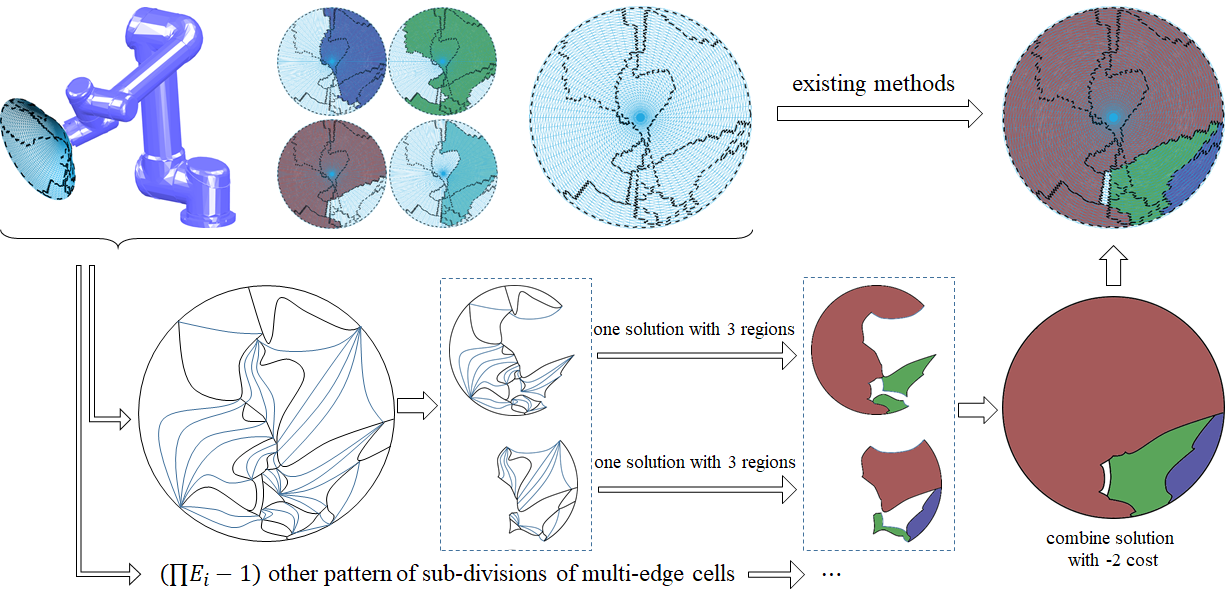
\includegraphics[width = 0.96\textwidth]{figures/hat_exp/fig_hat}
%\caption{\textcolor{blue}{What if I directly use the sub-graph in this experiment to be the demo figures of the above algorithm section? }}\label{fig:hat}
%\end{figure*}

\begin{figure}[t]
\centering
\subfigure[]{
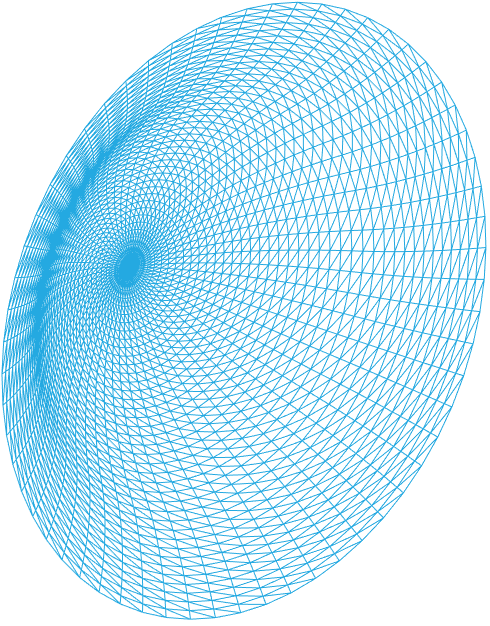
\includegraphics[width=0.15\textwidth]{figures/hat_exp/mesh}
}
\subfigure[]{
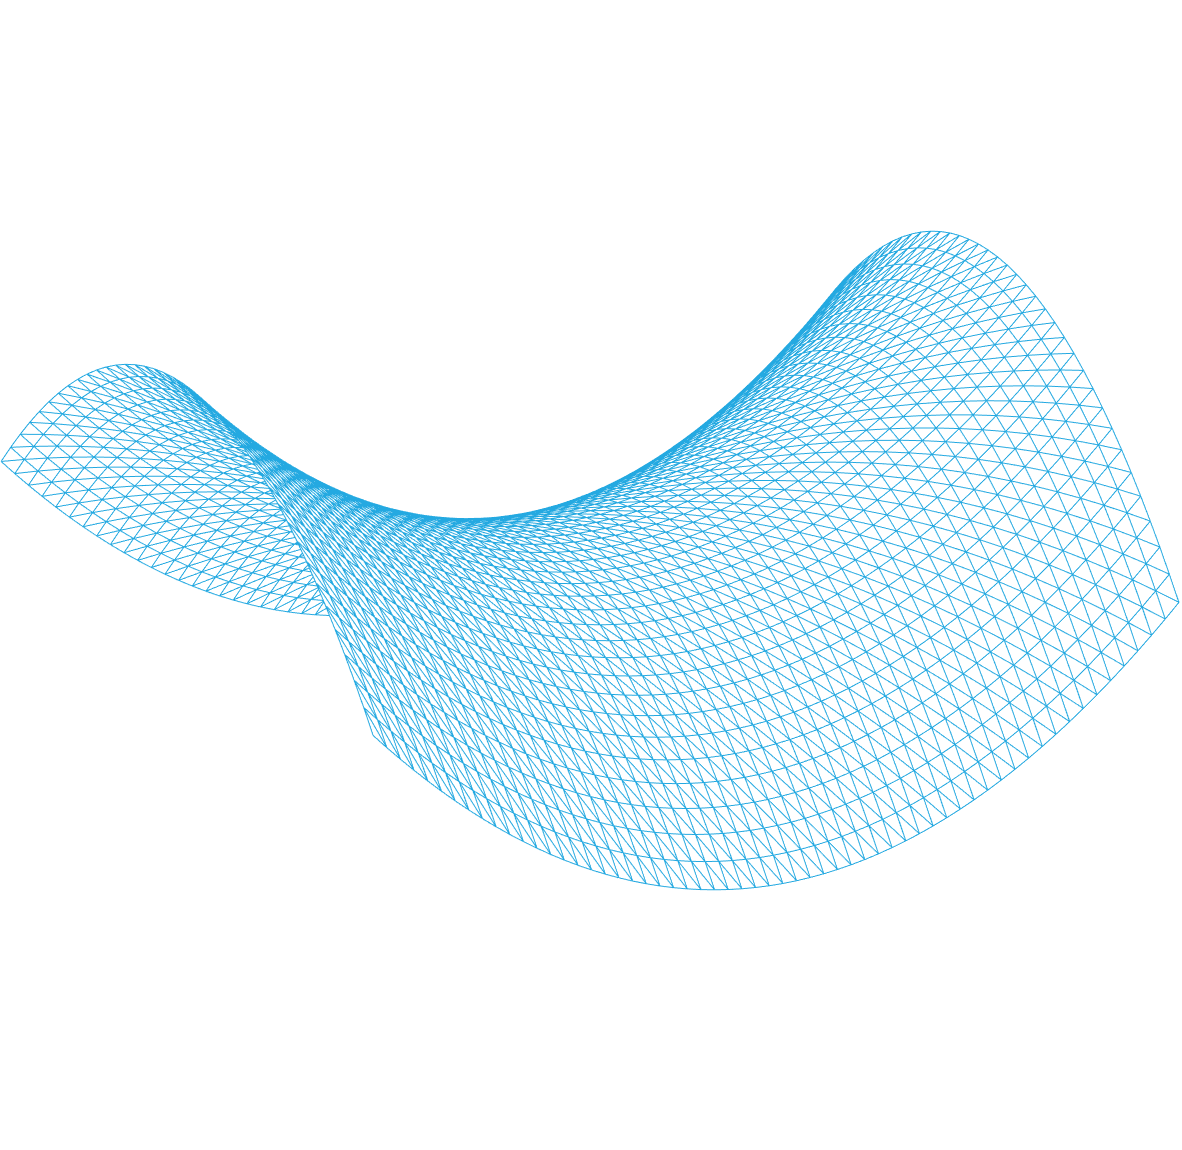
\includegraphics[width=0.15\textwidth]{figures/saddle_exp/mesh}
}
\caption{The objects used for illustration in Section \ref{section_results}. }\label{fig:object}
\end{figure}

\begin{figure*}[t]
\centering
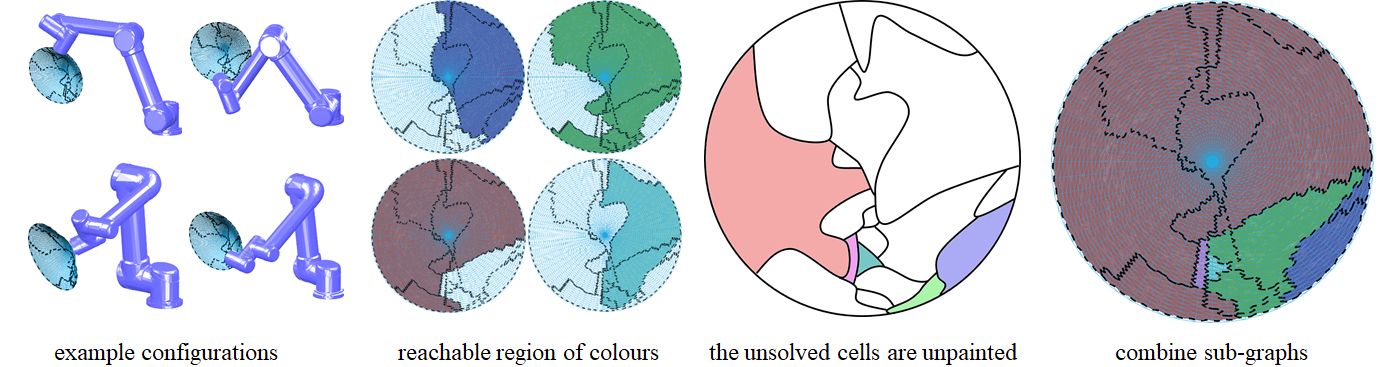
\includegraphics[width=0.96\textwidth]{figures/hat_exp/fig_hat_2}
\caption{The coverage task on a hat-shape object. The reachable area of different colours and one of their corresponding configurations are depicted. After painting all $1$-colour cells, the unsolved graph is exactly the same one as we have discussed in Section \ref{section_graph_separation}. }\label{fig:hat}
\end{figure*}
\begin{figure*}[t]
\centering
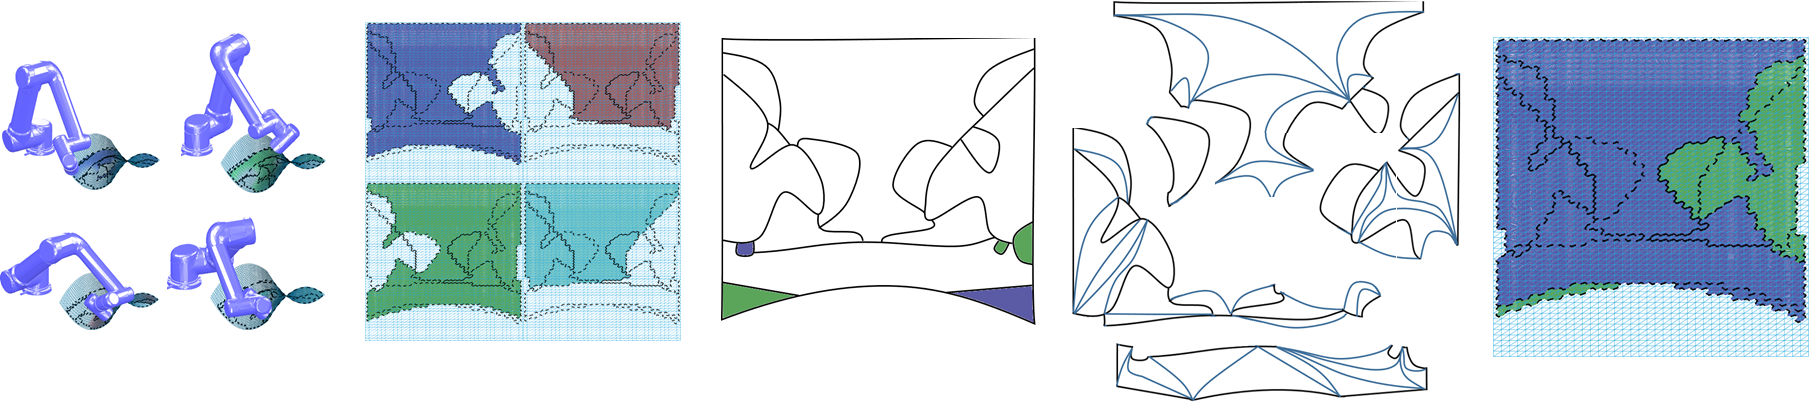
\includegraphics[width=0.96\textwidth]{figures/saddle_exp/comb}
\caption{The coverage task on a saddle surface. The reachable area of different colour and one of their corresponding configurations are depicted. After painting all $1$-colour cells, the unsolved grpah is separated into $5$ sub-graphs. Finally, all optimal solutions can be collected with 2 end-effector lift-offs.    }
\label{fig:saddle}
\end{figure*}

\section{Experimental Results}\label{section_experiment}
\label{section_results}

The proposed solution is tested experimentally by simulating the NCPP with a non-redundant manipulator (6 DoF Universal Robot UR5) on two arbitrarily shaped objects, one a hat-like concave semi-sphere (only one side is considered), and a saddle surface (only one side being considered also), as shown in Fig.~\ref{fig:object}.

\subsection{Optimal NCPP on a Hat-shape Object}
% <ty> Suddenly I notice that the demo figure is not illustrative. Will change
An illustration of the solving process for the hat-shape object is depicted in Fig.~\ref{fig:hat}. 
Four continuous sets of manipulator configurations are represented in blue, red, green and cyan colour separately. $1$-colour cells have been directly drawn to the graph. 
%Using existing algorithms~\cite{Yang2020Cellular}, the initial topological graph is directly enumerated. We need to iteratively decide whether keep/remove each topological edges, and choose colour for each (sub-)cells, leading to complexity as (\ref{equ:tmech}). One of the graph after cell sub-divisions is shown in Fig.~\ref{fig:hat}.  
The cell sub-divisions correspond to the description provided earlier in Fig.~\ref{fig:complicated_graph}.
For the algorithmic complexity there are $43$ cells. The possible colours of each cell are known. As for edges, there are $44$ unsolved edges (drawn in black) and $30$ manually created edges - enforced to be kept (drawn in blue). Plus $9$ edges which are connected to unreachable area (a fifth colour), which need not solving. Using the naive enumeration proposed in the literature, %~\cite{Yang2020Cellular} - we've repeated this too many times I feel
$35$ edges and all colours of all cells are enumerated, resulting in an algorithmic complexity described by 
\begin{equation}
{\color{red}2^{35}\times}
\begin{aligned}
&\overbrace{2\times2\times3\times2\times2\times2\times{\color{red}2\times2\times}}^{\textbf{all cells in sub-graph 1, shown in Fig.~\ref{fig:characteristic_string}}}\\
&2\times3\times3\times2\times2\times3\times2\times3\times2\times{\color{red}3\times}\\
&2\times2\times2\times2\times2\times2\times{\color{red}2\times}\\
&2\times3\times3\times4\times4\times{\color{red}3\times4\times}\\
&3\times3\times2\times3\times3\times4\times4\times{\color{red}3\times}\\
&3\times4\times3
\end{aligned}
\approx 1.2705\times10^{28}
\end{equation}
Please note there is a minor abuse of notation in the arrangement of the numbers above simply so that they can be easier to compared with the optimal solution below. 
%\begin{equation}
%2^{35}\cdot \underbrace{2\times 2\times \cdots \times 3}_{43 \mbox{ terms, number of colours}} \approx 1.2705*10^{28}
%\end{equation}

Using the proposed algorithm, the length of the boundary for each sub-graph is $6, 11, 9, 6, 10, 5$ respectively. The reader is referred to the sub-graph $1$  exammple
employed to discuss the process in detail in Sections~\ref{section_intersection} and~\ref{section_graph_separation}. Detail results for the others cases are ommited for lack of space, 
but follow the same process. 
The numberof colours for the boundary cells in each sub-graph is included in the multiplicative factor, so the algorithm complexity derives in the multiplication of 
the complexity of all sub-graphs, given by 
\begin{equation}
\begin{aligned}
&\overbrace{2\times2\times3\times2\times2\times2\times}^{\mbox{internal cells shown in Fig.\ref{fig:characteristic_string}}}\\
&2\times3\times3\times2\times2\times3\times2\times3\times2\times\\
&2\times2\times2\times2\times2\times2\times\\
&2\times3\times3\times4\times4\times\\
&3\times3\times2\times3\times3\times4\times4\times\\
&3\times4\times3
\end{aligned} \approx 4.2797\times10^{14}
\end{equation}

\subsection{Optimal NCPP on a Saddle-shape Object}
Another example is provided with the analysis of the outter shell of saddle-shape object. In this case the surface normal varies greatly as the end-effector moves 
along the surface, representing a challeging manipulator planning problem in adopting poses that would benefit the continuos coverage this paper is intererested in. 
The algorithmic complexity given cell sub-divisions is shown in Fig.~\ref{fig:saddle}. For the  naive enumeration case, the overall complexity is given by 
\begin{equation}
\begin{aligned}
&{\color{red}2^{47}*}~
\begin{aligned}
&2\times2\times2\times2\times2\times2\times2\times2\times2\times{\color{red}2\times}\\
&3\times2\times2\times2\times2\times2\times2\times \\
&~~~~3\times4\times4\times3\times2\times2\times2\times3\times{\color{red}3\times}\\
&3\times2\times2\times2\times2\times3\times3\times2\times{\color{red}2\times}\\
&4\times4\times4\times4\times4\times4\times3\times4\times{\color{red}4\times}\\
&3
\end{aligned}\\
&\approx 2.924\times10^{32}
\end{aligned}
\end{equation}

Applying the proposed algorithm, the complexity is reduced to
\begin{equation}
\begin{aligned}
&2\times2\times2\times2\times2\times2\times2\times2\times2\times\\
&3\times2\times2\times2\times2\times2\times2\times\\
&~~~~3\times4\times4\times3\times2\times2\times2\times3\times\\
&3\times2\times2\times2\times2\times3\times3\times2\times\\
&4\times4\times4\times4\times4\times4\times3\times4\times\\
&3\\
&\approx 4.3283\times10^{16}
\end{aligned}
\end{equation}

The overall results are gathered in Table~\ref{table:results} for easier comparison, collecting the substantial computational improvement in 
the number of edges for each problem ($35$ and $47$ repectively). As the geometry of the object of interest becomes more intricate, 
the benefit of the proposed scheme to be able to find paths with minimal discontinuities in joint-space with a reduced computational effort 
becomes also more apparent.
\begin{table}
\centering
\caption{Experimental results}
\begin{tabular}{ | c || c | c | c | c | }
 \hline
  Object  & \multicolumn{2}{|c|}{Number of Iterations} \\
 \hline
  						& Full enumeration~\cite{Yang2020Cellular}  &  Proposed Optimal \\
 \hline
 Hat-shaped ( Fig.~\ref{fig:hat})   	& $1.2705*10^{28}$    				&   $4.2797*10^{14}$\\
 \hline
 Saddle-shaped (Fig.~\ref{fig:saddle})					&   $2.924*10^{32}$  		&   	$1.0821*10^{16}$\\
 \hline
\end{tabular}
\label{table:results}
\end{table}


%\begin{table}
%\begin{tabular}{ | c || c | c | c | c | }
% \hline
%  Object  & \multicolumn{4}{|c|}{Solver} \\
% \hline
%  						& \multicolumn{2}{|c|}{Full enumeration~\cite{Yang2020Cellular}}  &  \multicolumn{2}{|c|}{Proposed Optimal} \\
% \hline
% 						&  $\Gamma$  & time(sec.)? other to compare? 	& $\Gamma$ & time?\\
% \hline
% Hat-shaped ( Fig.~\ref{fig:hat})   	& X    		& Y		&   X' 		& Y'\\
% \hline
% Other (Fig.~\ref{fig:saddle})					&  a  		& b   		& a'   		& b'\\
% \hline
%\end{tabular}
%\caption{Experimental results. Computational time calculated on a Pentium ... configuration machine.}
%\end{table}


\begin{comment}
Several representative simulation works have been implemented to validate the proposed algorithm on challenging  arbitrarily-shaped objects.
% the optimal non-revisiting coverage planning path is solved. 
Fig. \ref{fig_mobius_exp} presents the solution of polishing a Mobi\"{u}s strip, whose surface is non-orientable. The manipulator is required to maintain the EE normal to the surface for proper operation simulating a contact task such as polishing. This is rather challenging in this case 
since the strip is twisted, hence the orientation of the normal vector varies over the full $2\pi$ rads. However, the proposed algorithm 
is able to come up with a configuration mapping leading to an optimal solution where only $1$ lift-off is required over the entire object.

Fig. \ref{fig_ring_exp} depicts the process of covering the surface of a ``swimming'' ring, another closed surface with no boundary. 
This is a particularly challenging case, it can be seen how the topological graph is formed by cells that are all multiply-connected, 
yet the proposed algorithm is able to come up with an effective solution with a single configuration discontinuity to the NCPP problem. 

The examples in Fig.~\ref{fig:hill_multiply_conn}, Fig.~\ref{fig_hill_exp_0_10} and Fig.~\ref{fig_hill_exp_0_16} illustrate the solutions of covering a ``hilly terrain" with varying degrees of desirable manipulability~\cite{Yoshikawa1990Translational}. 
For a given configuration (colour) cell, the manipulability is explicitly depicted brighter for increasing manipulability for the given configuration. The threshold  varies from a minium of $0.06$ (Fig.~\ref{fig:hill_multiply_conn}) to at least $0.10$ (Fig.~\ref{fig_hill_exp_0_10}), up to at least $0.16$, the maximum where a solution can be found for the object (in Fig.~\ref{fig_hill_exp_0_16}).
As one would expect, a sharp reduction in the reachable area is observed as the manipulability tightens 
(mainly due to the limited mobility of the wrist-flipped configurations, shown in the bottom two configurations 
in Fig.~\ref{fig:manip_010_configs}), causing large fluctuations in the structure of the resulting cells and topology graphs. When the threshold goes to $0.16$, most of the kinematic-valid wrist-unflipped configurations are no longer valid, as depicted in Fig.~\ref{fig_hill_exp_0_16}. 
\end{comment}

\section{Conclusions}
An advancement to efficiently solve non-repetitive coverage tasks with a non-redundant manipulator is proposed in this work. 
The core concept is the introduction of topological intersections and intersection-free graphs, which permits the separation of a graph 
into sub-graphs at the points where the multiplicity of optimal solutions originate. 
The implicit enumeration of these intersections when the graphs are recombined in search of the full solution derive in a mathematically proven exponential improvement in the order of $2^N$, $N$ representing the number of topological edges in the graph. This is particularly relevant for intricate task-space graphs,
where an exhaustive search for solutions with all the cells and edges is unattainable. 
Comprehensive experimental results with step-by-step derivations to illustrate the proposed algorithm are supplied that demonstrate the validity of the novel scheme. 
\label{section_conclusion}


%% Use plainnat to work nicely with natbib. 

%\newpage 

\bibliographystyle{plainnat}
\bibliography{faster_solution_RSS21}

\end{document}


